\documentclass[12pt]{article}
\setlength{\topmargin}{-0.5in}
\setlength{\oddsidemargin}{0.33in}
\setlength{\textheight}{9.0in}
\setlength{\textwidth}{6.0in}

\usepackage[utf8]{inputenc}
\usepackage[dvipsnames]{xcolor}
\usepackage{amsmath,hyperref,graphicx,caption,subcaption,float,pifont}
\captionsetup{belowskip=0pt}
%\usepackage[ruled]{algorithm2e}
\usepackage[style=numeric,backend=biber]{biblatex}
\usepackage{tikz}
\def\checkmark{\tikz\fill[scale=0.4](0,.35) -- (.25,0) -- (.25,.15) -- cycle;}
\addbibresource{bibliography.bib}

\title{Chimeras in a Fragmented Landscape}
\author{Alison Peard}
\date{March 2021}

\begin{document}
\tableofcontents
\maketitle

\section{Introduction}\label{section:intro}
\colorbox{red}{fix tenses- present tense}
Ecosystems around the world are being increasingly fragmented by human activity due to agriculture, logging and urban expansion \cite{lucey2014,laurance2011} \colorbox{yellow}{ref for this needed}. Ecologists and conservationists want to understand how the preservation of biodiversity can be balanced with continuing human progress and development. \\ A good example of this is palm oil production; oil palm is an extremely lucrative crop and its production motivates the deforestation of the Amazon rainforest where fertile soils lead to high yields \cite{meijaard2018oil}. As the industry continues to expand with increasing demand it is important that it does so in a way that minimises biological destruction. International organisations and projects such as the Roundtable for Sustainable Palm Oil and the SEnSOR project work hard to test the effectiveness of different techniques to minimise the biodiversity loss caused by oil palm plantations \cite{scriven2019testing}. \\ \\ In order to support the conservation of any habitat as effectively as possible we need to understand the complexities of how fragmentation impacts population dynamics in an ecosystem. How will the previously continuous ecosystem react to a new road which splits it in two? Will populations increase or decrease or will something more unexpected occur?  \\ \\ \colorbox{yellow}{Rainforest fragmentation .png here} \\ \\ This project combines dynamical systems theory with network science and abstracts a general ecosystem to a network of coupled oscillators with each oscillator exhibiting identical intrinsic dynamics. Thus, each node represents a fragmented patch of said ecosystem. In particular, we seek to understand what contributes to complete synchronisation across all patches, a phenomenon known as the Moran effect, which can lead to heightened risk of species-wide extinctions \cite{hansen2020moran}. We look for combinations of habitat features that give rise to chimera, a spatiotemporal pattern that has inspired extensive research since it's discovery by Kuramoto and Battogtokh \cite{bera2017chimera}. Is it better to have lots of well-connected smaller fragments, for example, or are a fewer larger fragments more conducive to robust populations? We will explore how different types of fragmentation affect ecosystems by looking at a selection of network topologies and parameters and observing the behaviours that are produced. The three features we will explore are network structure, habitat patch size and connectivity strength between patches. The former we modify via the networks adjacency matrix while the latter two features are represented by model parameters.

\section{The Rosenzweig MacArthur Model}\label{section: model intro}
The Rosenzweig-MacArthur model \cite{rosenzweig1963} is a simple predator-prey model that models the dynamics of some prey species $x(t)$ and some predator species $y(t)$. The population density of the prey will increase according to some constant birth rate $r$ and is limited by the carrying capacity of its habitat $k$ which represents what size population a patch can support and could be indicative of patch size, food availability or the combination of any number of environmental conditions. \\
The population of the prey is assumed to only decrease as it is consumed by predation and this is represented by the last term of the first equation in (\ref{eq:RMT single}). This term is a function of both population densities and the effectiveness of the predators which is represented by $m$. A predator can only consume so many prey at a time, so for each predator the benefits of an abundant prey population begin to max out as $x$ becomes very large. This is achieved mathematically by the Holling Type II functional response $\frac{x}{1+x}$, which asymptotically approaches $1$ as $x \to \infty$. The population density of predators will increase proportional to this term and decrease proportional to some constant death rate, $c$. \\
The non-dimensionalised model becomes,
\begin{align}
    \dot{x} &= r x \left(1 - \frac{x}{k}\right) - m \frac{x y}{1+x} \\
    \dot{y} &= -c y + m \frac{x y}{1 + x} .
\end{align}\label{eq:RMT single}
This system has three equilibrium points,
\begin{align*}
    (x^*,y^*) =  \bigg\{ (0,0), (k,0),(\bar{x},\bar{y}) \bigg\}
    \end{align*}
where,
\begin{align}
(\bar{x},\bar{y}) = \Big(\frac{-c}{c-m},\frac{-cr - ckr +kmr}{k(c-m)^2}\Big).
\end{align} \ref{eq: coexistence equilibrium}
We are most interested in the stability of $(\bar{x},\bar{y})$ because this is the only situation where both predator and prey coexist.
\colorbox{yellow}{fill these in}.
Using linear stability analysis we find that
\begin{enumerate}
    \item the origin $(0,0)$ is a saddle-point for all $x$ with instability in the \colorbox{yellow}{CHECK DIRECTION}
    \item FIND THE LSA YOU DID
    \item the coexistence equilibrium bifurcates from a saddle to a stable node / spiral at $k= \frac{c}{m-c} $ before undergoing a Hopf bifurcation creating a stable spiral at $k = \frac{2c}{m-c}\left(\frac{m r}{\bar{y}(c-m)^2 - mr}\right)$.
\end{enumerate}

\begin{figure}[H]
    \begin{subfigure}[b]{0.5\linewidth}
        \centering
        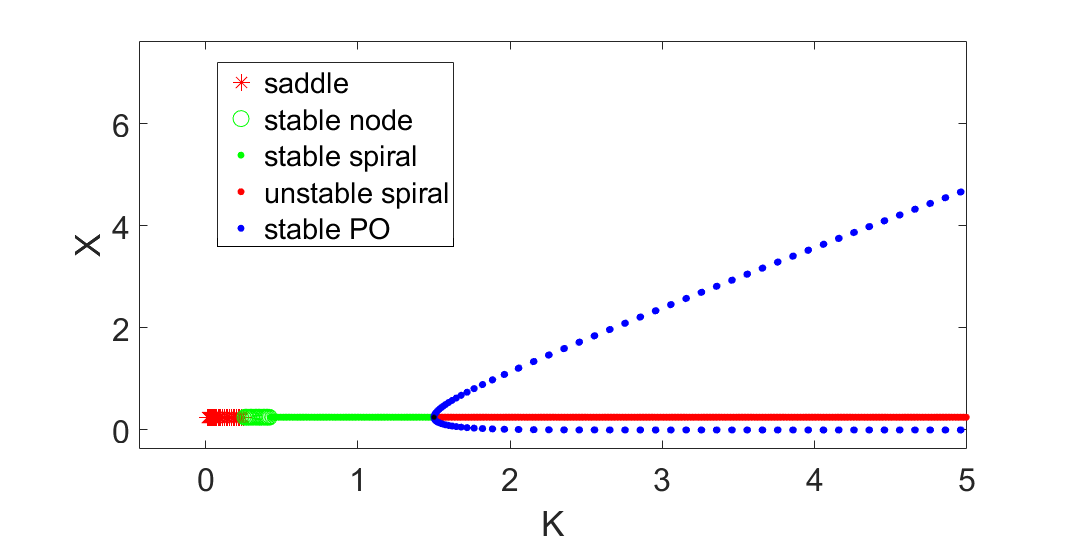
\includegraphics[width=\textwidth]{RM Model/periodicorbitbranch.png}
        \caption{Branch of the periodic orbit in the phase plane.}
        \hfill
    \end{subfigure}
    \begin{subfigure}[b]{0.5\linewidth}
        \centering
        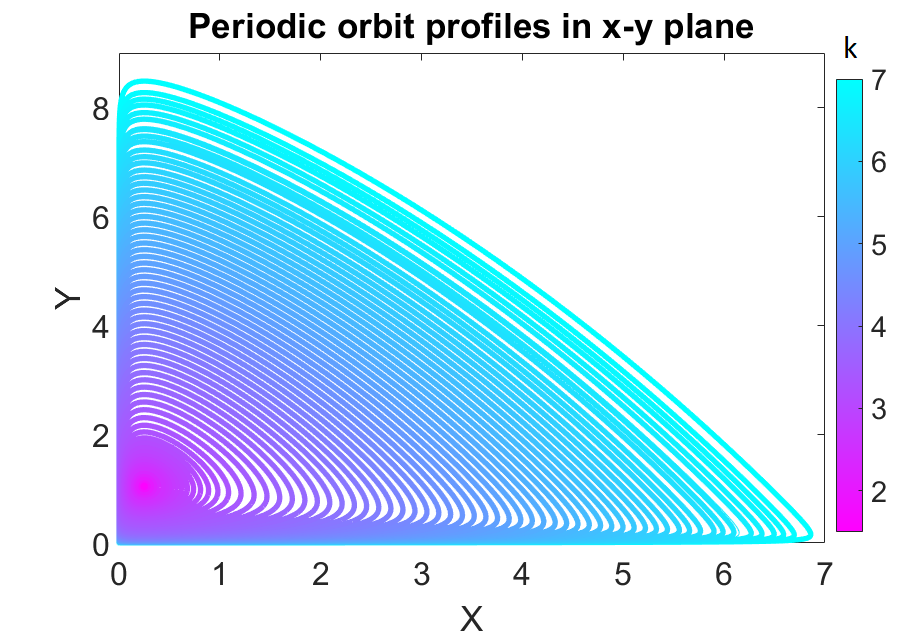
\includegraphics[width=\textwidth]{RM Model/periodicorbitprofiles.png}
        \caption{Profile of the periodic orbit after the Hopf bifurcation shows the paradox of enrichment emerging as $k$ increases.}
    \end{subfigure}
\end{figure}\label{fig: paradox of enrichment}

\subsubsection{The paradox of enrichment}\label{section: paradox of enrichment}
Honing in on the dynamics of the limit cycle that are produced by the Hopf bifurcation, Figure \ref{fig: paradox of enrichment} shows a cross section of the periodic orbit for increasing $k$-values. Observe how increasing $k$ increases the amplitude of oscillation which in turn causes the populations to plummet towards zero regularly. This slightly counter-intuitive result, termed the paradox of enrichment by Rosenzweig in 1971 \cite{gilpin1972enriched} describes how an overabundance of resources can actually destabilise a system and lead to extinctions. There is plenty of debate as to whether this paradox hold in the real world \cite{jensen2005paradoxes} however some recent studies do appear to have observed it, occurring as a result of eutrophication in lakes and algal populations \cite{cottingham2000increased, jensen2005paradoxes}. This paradox will motivate our interest in synchronisation and incoherence later.

\subsection{Extension to a system of populations}\label{section: extension to system of populations}
To explore the concept of fragmentation, we construct a system of habitat patches as a network of coupled Rosenszweig-MacArthur models.
\begin{align}
    \dot{x_i} &= r x_i (1 - \frac{x_i}{k}) - m \frac{x_i y_i}{1+x_i} \\
    \dot{y}_i &= -c y_i + m \frac{x_i y_i}{1 + x_i} + \sigma \Sigma_{j=1}^nA_{ij}(y_j - y_i).
  \end{align}\label{fig: RMT system}
\noindent
Patches are said to be coupled if there is migration of predators between them and this is represented by the additional term on the second differential equation, where $A_{ij}$ is a network adjacency matrix and $\sigma$ is the parameter for coupling strength or predator migration rate. This term represents a \textit{consensus dynamics} setup, where each node adjusts to reduce the difference between itself and its neighbours \cite{lambiottenotes}. If $\dot{y}(t)$ were a function of this term alone then the system would settle into a global 'consensus state' where all nodes would take the average value of the initial conditions.
The simplification of only considering predator movement between patches can justified by primarily considering predator-prey systems where the prey are slow moving animals or plants. In the natural world this is often the case. \colorbox{yellow}{reference?} \\
Hence, varying the network topology via it's adjacency matrix and coupling via parameters serves as an abstraction of differing types of fragmentation in the natural world. \\

\subsubsection{A note on visualising network dynamics}
It is convenient to visualise spatiotemporal dynamics of these systems using heatmaps with node index on the $x$-axis and time on the $y$-axis. For a 1-d lattice this is straightforward, nodes are plotted with each of their neighbours on either side. Since the network topologies in question are not always so simple, in other cases we must flatten our node to a simple array in order to plot it. Hence it will not always be clear from the heatmaps which nodes are connected neighbours. Since we are seeking only to identify whether or not certain behaviours are actually present, however, this is justified because the presence of chimera or synchronisation will still be apparent from this set up. Further analysis or grouping of nodes into different regions based on these plots shouldn't be attempted without a supplementary understanding of the network topology however.

\section{Emerging Incoherence and Chimeras}\label{section:chimeras}
\subsection{The paradox of enrichment (revisited)}
Now considering systems instead of just single habits, it is useful to return to the paradox of enrichment as in Section \ref{section: paradox of enrichment} and notice an important consequence. If a system of nodes is exhibiting strong spatial correlation and oscillation in synchrony, hypothetically, then these dangerously high amplitude oscillations may spread across the system and lead to cascading extinctions across a much larger area. This is one of the reasons that we are particularly interested in understanding when a system will oscillate with strong synchrony and when patches will display more independent behaviour. These more incoherent system dynamics tend to be more transient that steady states such as the prey-only equilibrium discussed in Section \ref{section: model intro}.

\subsection{Transient dynamics}
Transient dynamics occur as a system shifts from one state to another and theses transients may occur quickly or last over extremely long time-periods. It is also possible for a system to remain in a transient state indefinitely \cite{transientsweb}  on asymptotic steady state dynamics \cite{hastings2004transients,hastings2018transient}. This is a rather significant simplification seeing as ecological data is usually collected over short time periods so it cannot really be assumed that the systems have settled into their asymptotic steady states.

\subsection{Chimeras}
A particularly interesting transient behaviour occurs when a system splits into coexisting regions of coherence and incoherence. This phenomenon, which was christened "chimera" by Abram and Strogatz in 2004 is defined as follows: \textit{"a chimera state is a spatiotemporal pattern in which a system of identical} [coupled] \textit{oscillators is split into coexisting regions of coherent and incoherent oscillation"}.

\begin{center}
 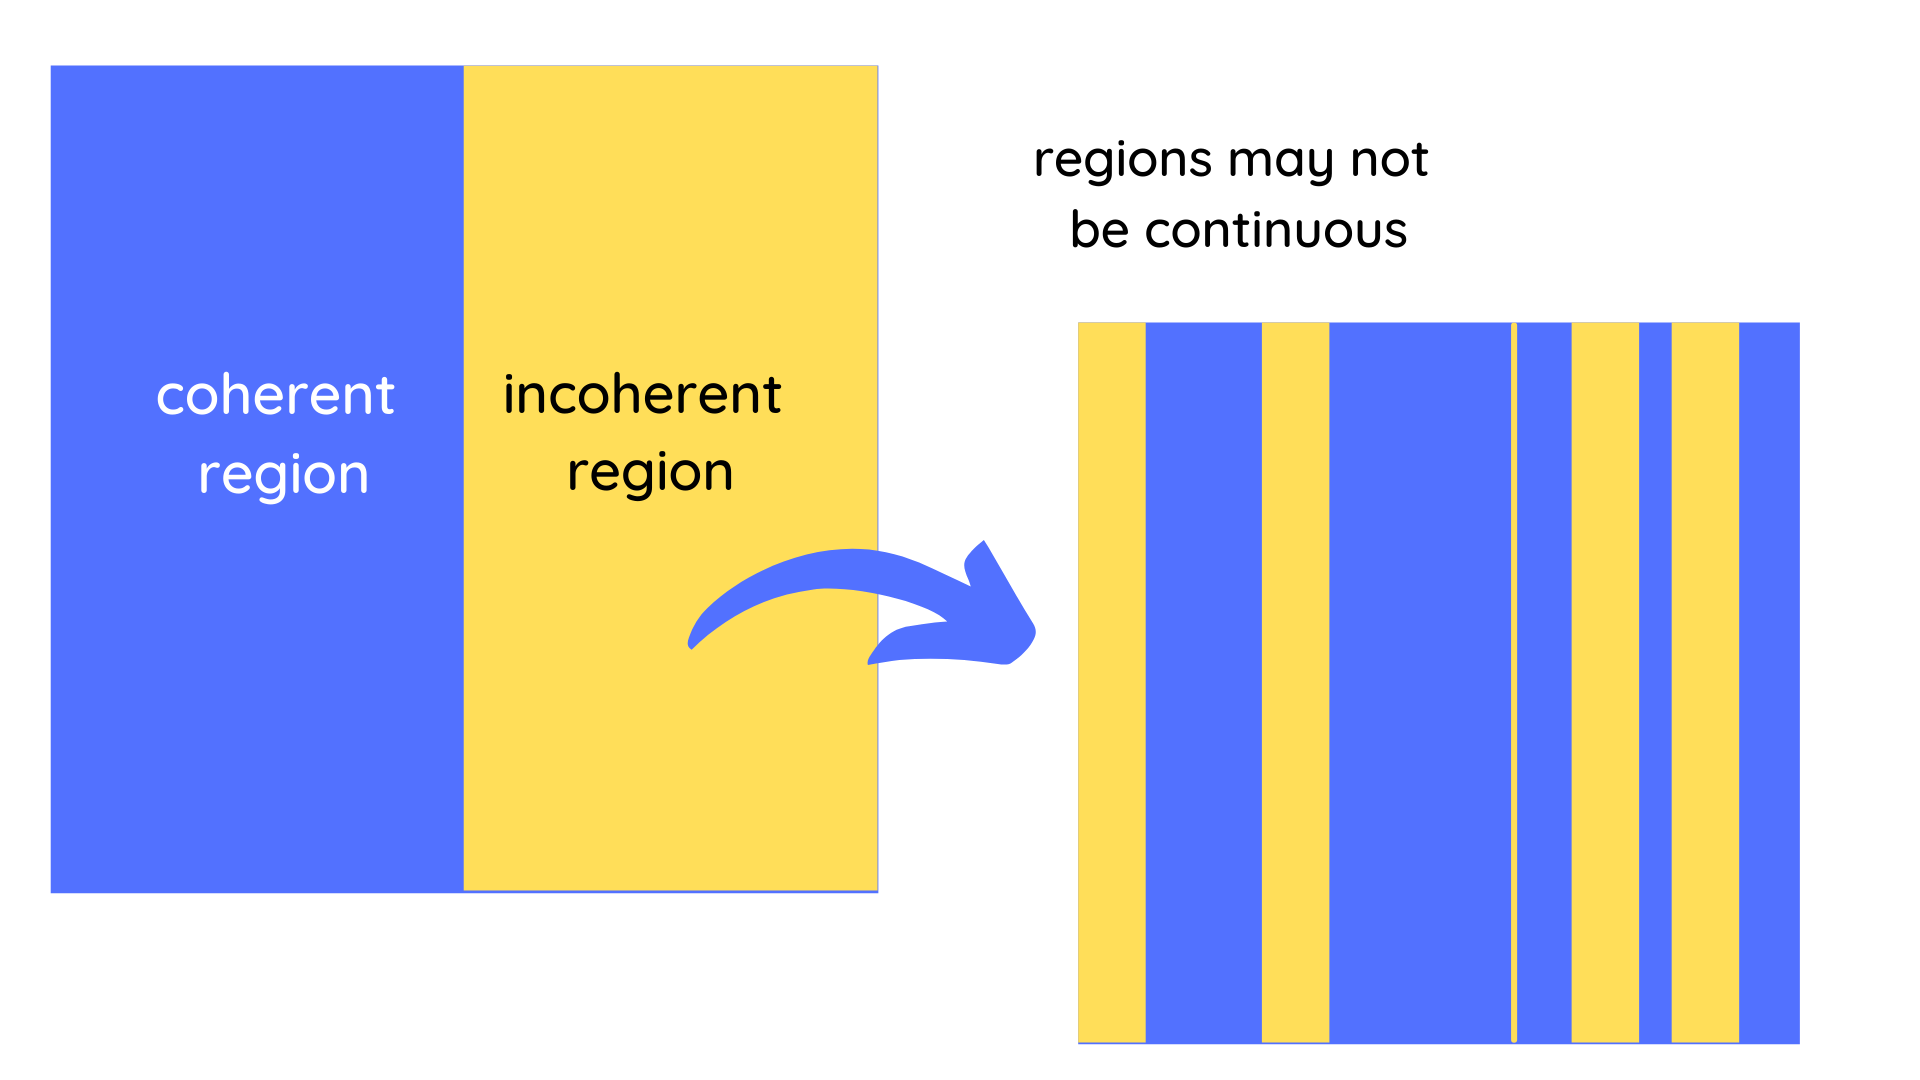
\includegraphics[width=0.6\textwidth]{General Diagrams/chimera intro.png}
\label{fig: chimera diagram}
\captionof{figure}{A system in chimera will have a coherent and an incoherent region.}
\end{center}
Since then it has been extensively researched and many forms of chimera discovered, but many of the definitions are not set in stone and may vary from paper to paper \cite{haugland2021changing}. The main definitions used throughout this paper were chosen to align with the those used by Dutta and Banerjee in their 2015 paper \textit{Spatial coexistence of synchronized oscillation and death: A chimeralike state} and Zakharova in \textit{Amplitude chimeras and chimera death in dynamical networks} \cite{dutta2015, zakharova2015}. Chimera types worth highlighting and of particular relevance are amplitude chimera, chimeralike synchronised oscillation and death (CSOD) and mixed state amplitude chimera and death \cite{dutta2015, zakharova2015}. For consistency with the language of these papers, we allow the term 'death state' to imply oscillation death rather than population death and any node that is in a steady state can be considered as in a death state whether or not its value is zero. \\ \\

\begin{figure}[h]
\centering
\begin{subfigure}[b]{0.4\textwidth}
    \centering
    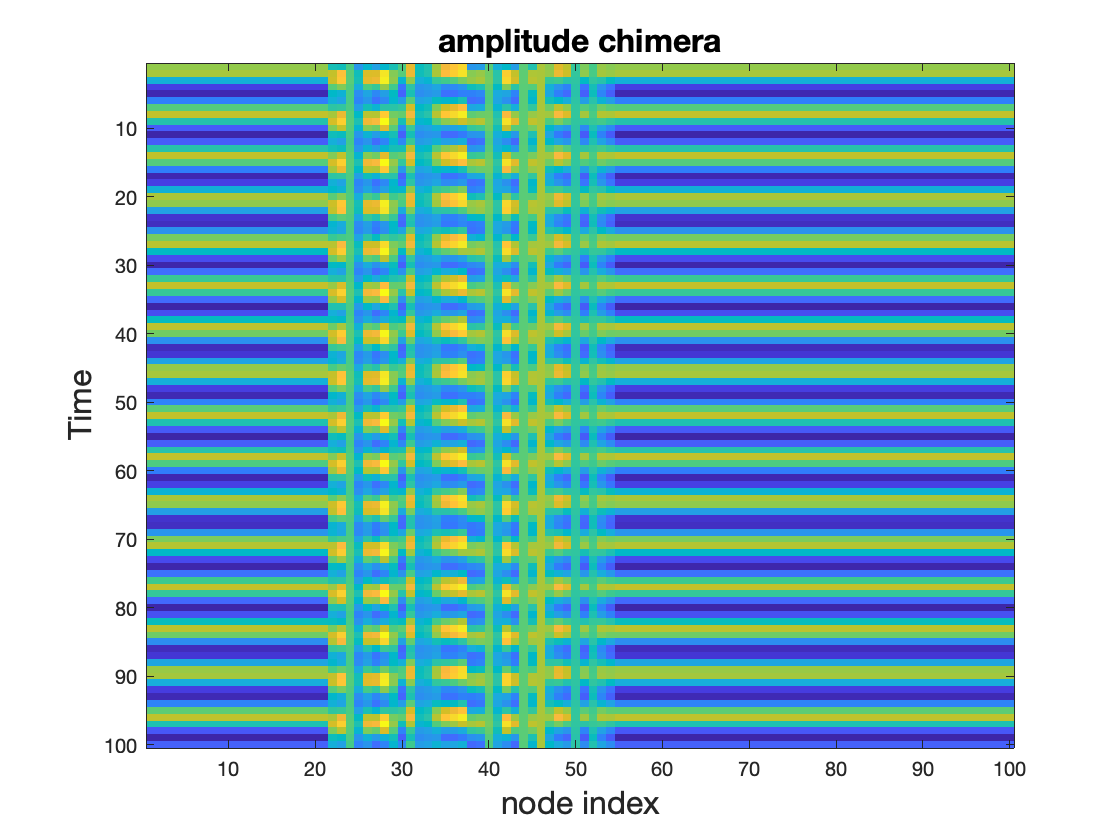
\includegraphics[width=\textwidth]{General Diagrams/amplitude chimera.png}
    \caption{Amplitude chimera }
    \label{fig: amplitude chimera}
\end{subfigure}
\hfill
\begin{subfigure}[b]{0.4\textwidth}
    \centering
    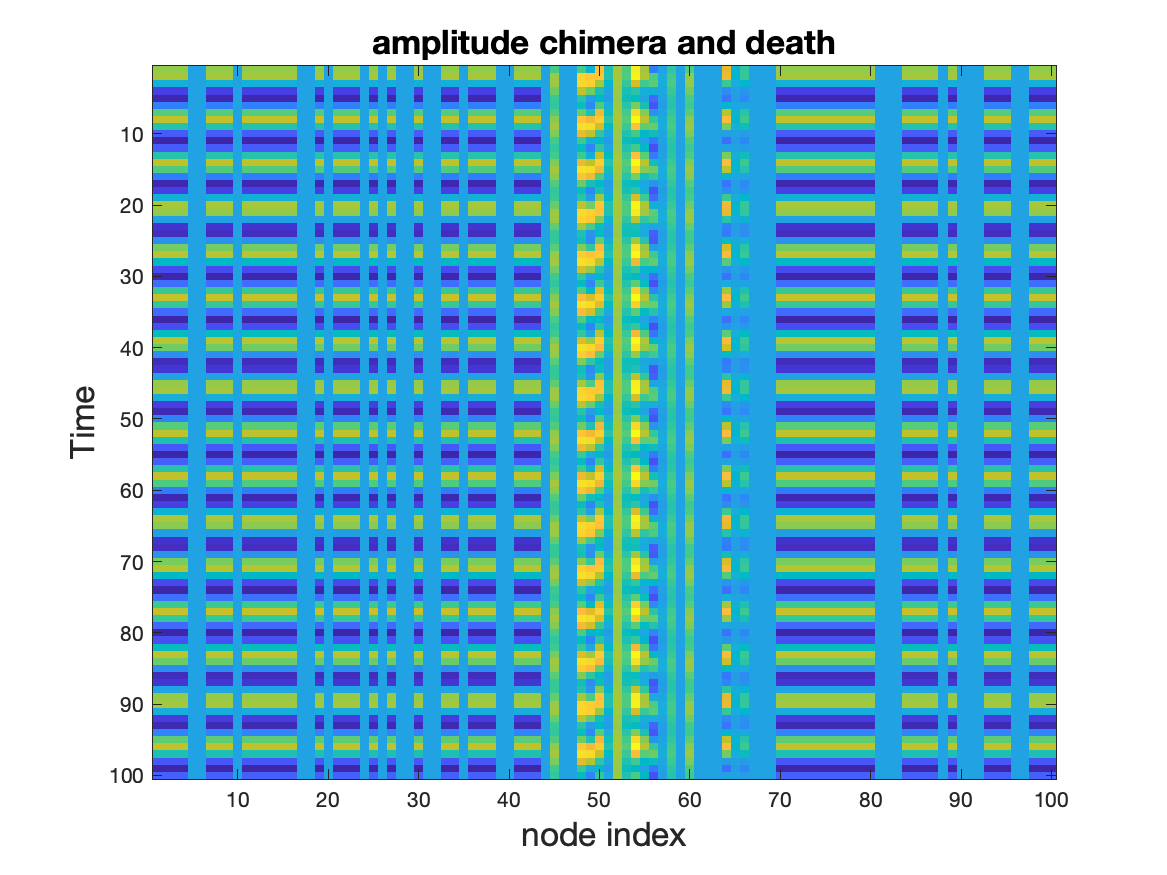
\includegraphics[width=\textwidth]{General Diagrams/amplitude chimera and death.png}
    \caption{AC and death }
    \label{fig:ac and death}
\end{subfigure}
\hfill
\begin{subfigure}[b]{0.4\textwidth}
    \centering
    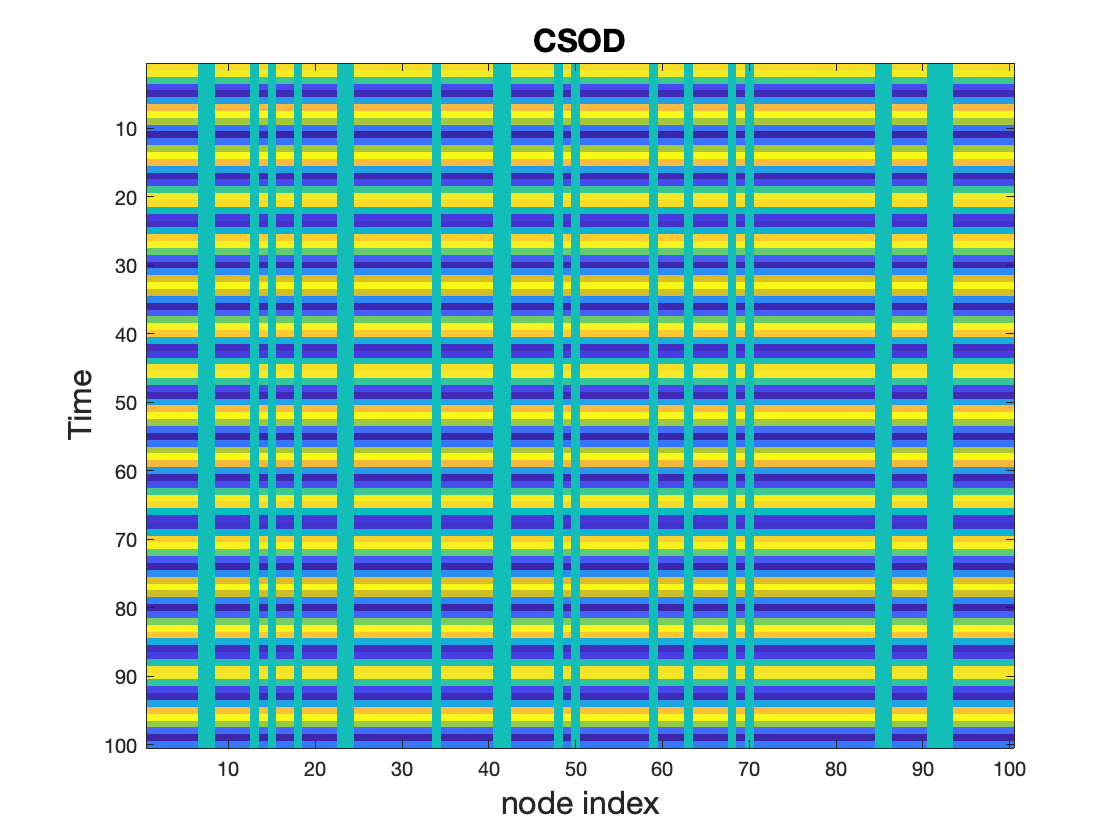
\includegraphics[width=\textwidth]{General Diagrams/CSOD.png}
    \caption{Chimeralike synchronised oscillations and death}
    \label{fig: CSOD}
\end{subfigure}
\hfill
\end{figure}

Amplitude chimera (Figure \ref{fig: amplitude chimera}) occurs when nodes in the coherent region oscillate in synchrony and nodes in the incoherent region have incoherently varying amplitudes. In all regions the phases of oscillation are correlated and frequencies are the same. None of the nodes will be in death states though some oscillations may have very low amplitude. CSOD (Figure \ref{fig: CSOD}) is observed when most of the nodes oscillating in synchrony but the system is interspersed randomly with death states. Lastly, the amplitude chimera and death state \ref{fig:ac and death} occurs when nodes are oscillating with amplitude chimera but the system is interspersed with death states.

\subsubsection{Using a classifier}
To efficiently explore these definitions across a wide range of network topologies and parameters it was useful to create an automatic classifier. This classifier is described in pseudo-code in the appendix \ref{appendix:classifier}. Using this classifier it is possible to quickly explore large parameter spaces for different networks.

\section{Exploring Network Topologies}\label{section:network topologies}
The effects of various degrees of nonlocal coupling in a habitat network will be explored using the concept of \textit{link distance}. Link distance $l$ here will mean the furthest away node another node can be connected to. If one were to draw a circle of radius $l$ around any node then it would be connected to all the nodes which lie within that circle. Beginning with a 16-node lattice, connections between nodes are added according to increasing link distance - increasing the amount of nonlocal coupling in the network.
\begin{figure}[h]
    \centering
    \begin{subfigure}[b]{0.4\linewidth}
    \centering
    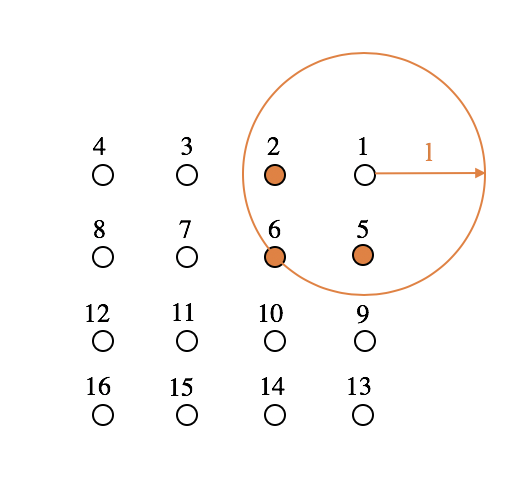
\includegraphics[width=\textwidth]{Xinzhu Section/link_dis_1.png}
    \caption{Link distance $l=\sqrt{2}$.}
    \end{subfigure}
    \hfill
    \begin{subfigure}[b]{0.4\linewidth}
    \centering
    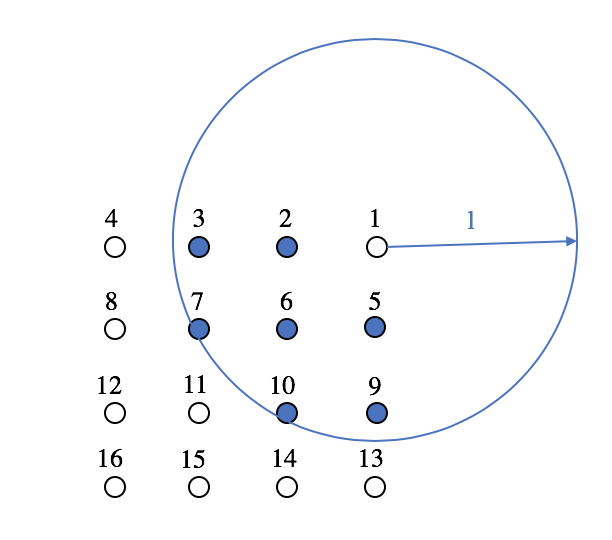
\includegraphics[width=\textwidth]{Xinzhu Section/link_dis_2.png}
    \caption{Link distance $l=\sqrt{2}$.}
    \end{subfigure}
    \label{fig:link distances}
\end{figure}
\noindent
Below $k=1.5$ the systems will all be in death states. This aligns with the Hopf bifurcation that occurs at this value for the single node system discussed in Section \ref{section: model intro}. We see these death states appear for up to $k$ as large as $k=2$ in the network and above this value various forms of coherent and incoherent oscillation occur.

\begin{figure}[h]
    \centering
    \begin{subfigure}[b]{0.4\linewidth}
    \centering
    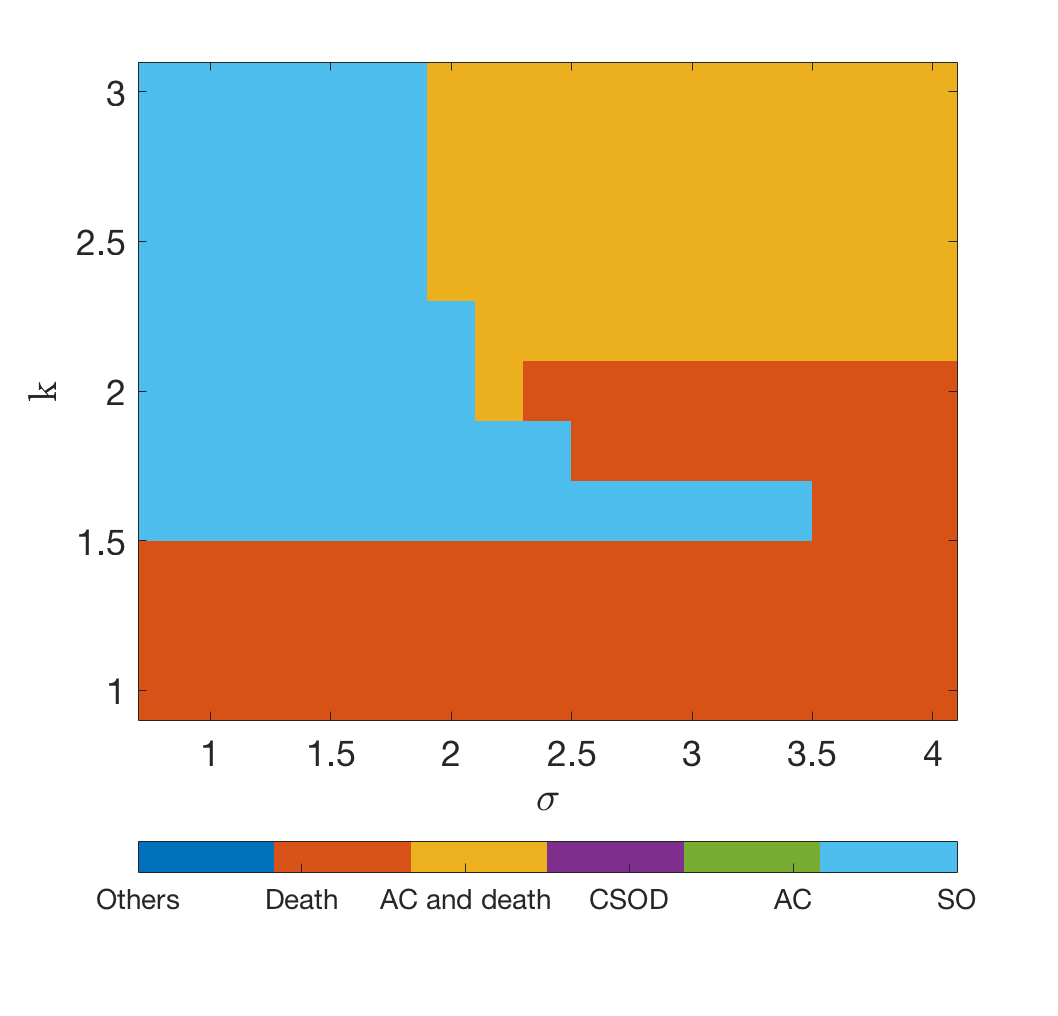
\includegraphics[width=\textwidth]{Xinzhu Section/2dlat16_1.png}
    \caption{Link distance $l=1$.}
    \end{subfigure}
    \hfill
    \begin{subfigure}[b]{0.4\linewidth}
    \centering
    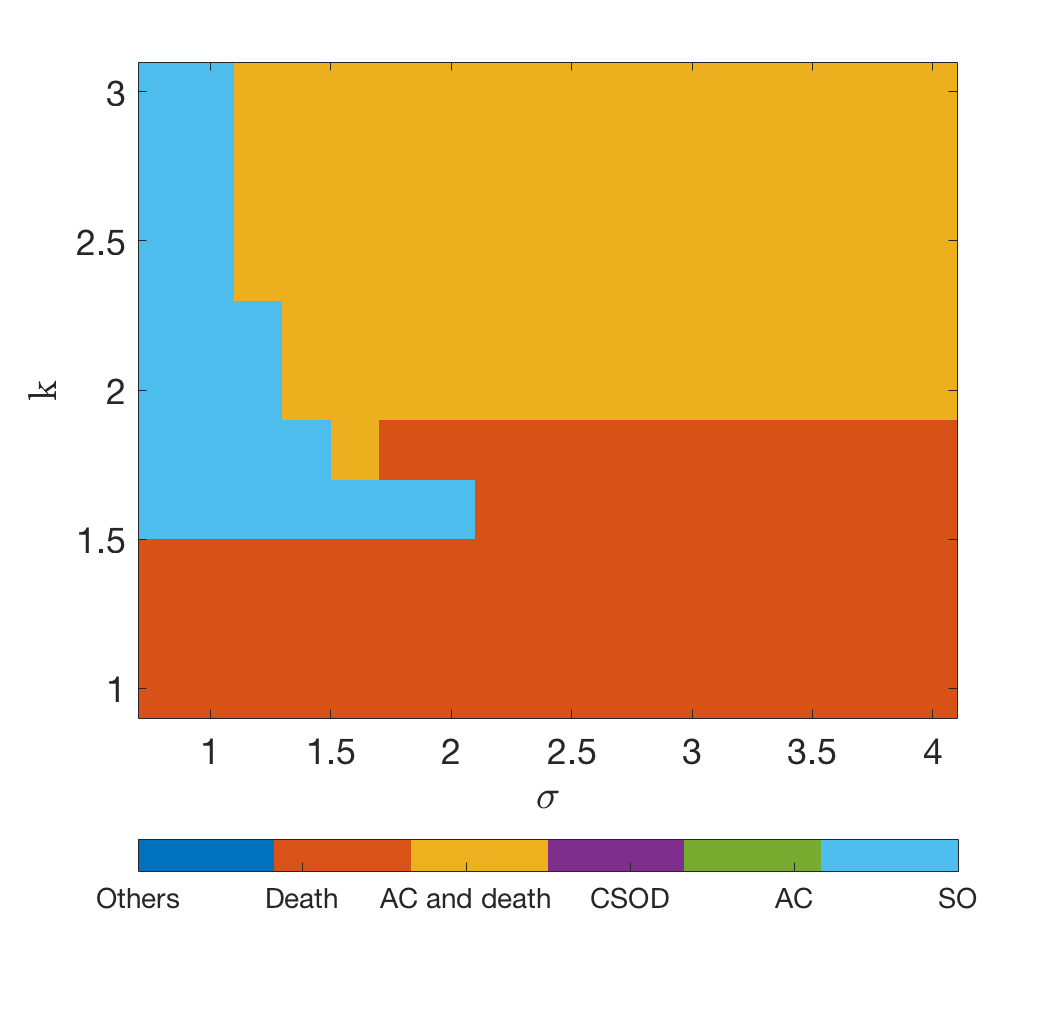
\includegraphics[width=\textwidth]{Xinzhu Section/2dlat16_sqrt(2).png}
    \caption{Link distance $l=\sqrt{2}$.}
    \end{subfigure}
    \label{fig:a link distances and parameter searches}

\end{figure}
\noindent For each link distance, carrying capacity $k$ is explored within the interval $[1,3]$ and migration rate $\sigma$ lies in the range $[0.8,4]$. As $l$ increases from $1$ to $\sqrt{5}$ the range of values for which synchronous oscillations occur decreases systematically, and the death state and the more incoherent amplitude chimera and death state become dominant. As $l$ continues to increase to $\sqrt{18}$ the amplitude chimera and death region is gradually replaced by CSOD behaviour as the synchrony between the nodes increases again. This is interesting as both synchronous oscillations and CSOD are more coherent than the mixed amplitude chimera and death state and implies that for quite low and quite high levels of nonlocal coupling the system is more synchronised than at intermediate levels.

\begin{figure}[h]
    \centering
    \begin{subfigure}[b]{0.4\linewidth}
    \centering
    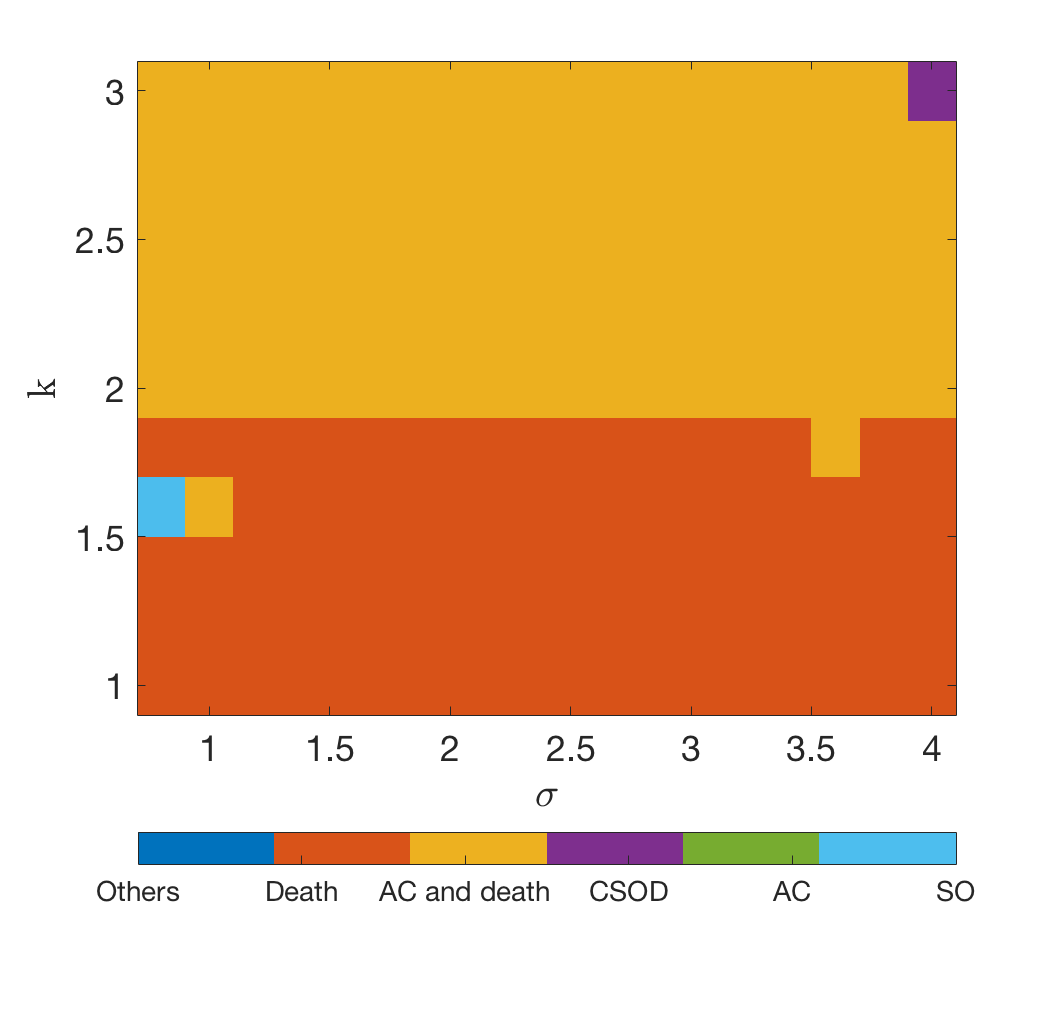
\includegraphics[width=\textwidth]{Xinzhu Section/2dlat16_sqrt(5).png}
    \caption{Link distance $l=\sqrt{5}$.}
    \end{subfigure}
    \hfill
    \begin{subfigure}[b]{0.4\linewidth}
    \centering
    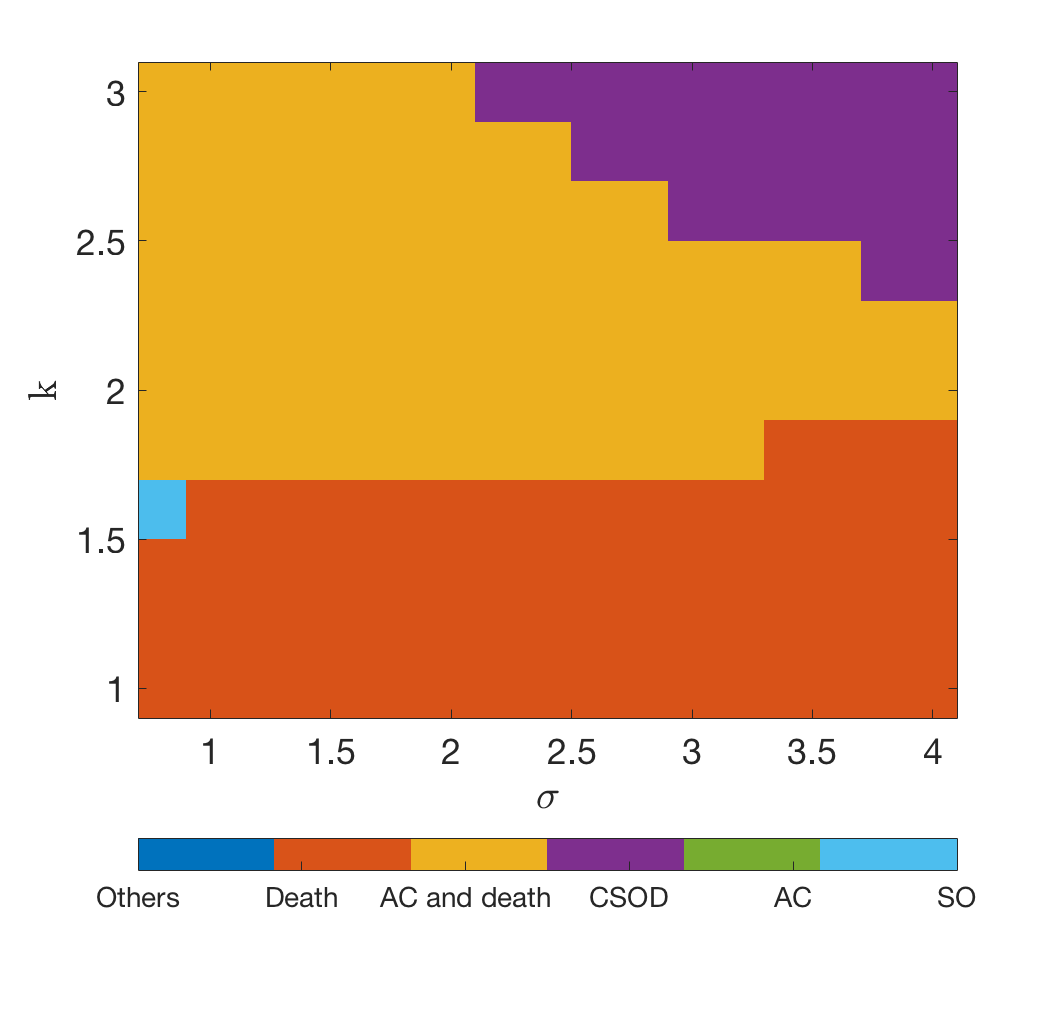
\includegraphics[width=\textwidth]{Xinzhu Section/2dlat16_sqrt(8).png}
    \caption{Link distance $l=\sqrt{8}$.}
    \end{subfigure}
    \hfill
    \begin{subfigure}[b]{0.4\linewidth}
    \centering
    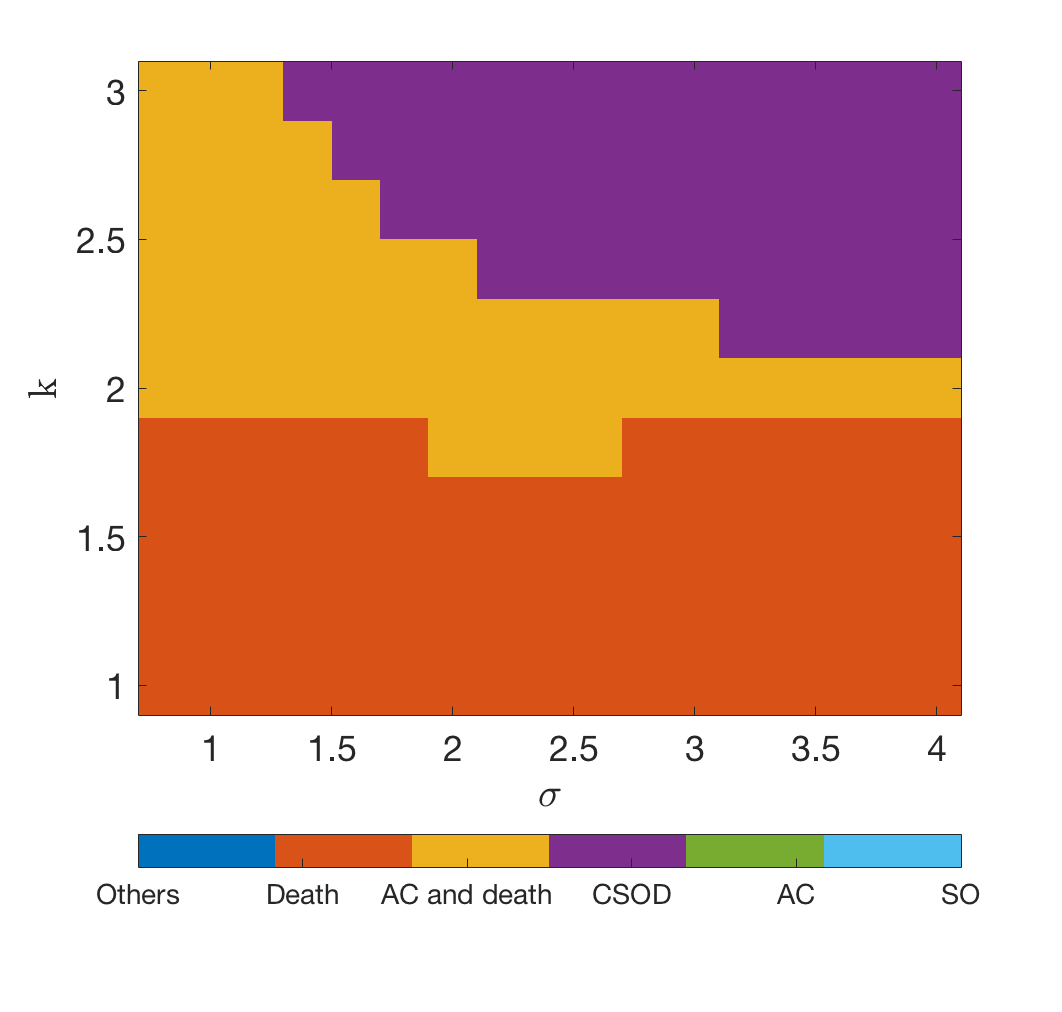
\includegraphics[width=\textwidth]{Xinzhu Section/2dlat16_sqrt(10).png}
    \caption{Link distance $l=\sqrt{10}$.}
    \end{subfigure}
    \hfill
    \begin{subfigure}[b]{0.4\linewidth}
    \centering
    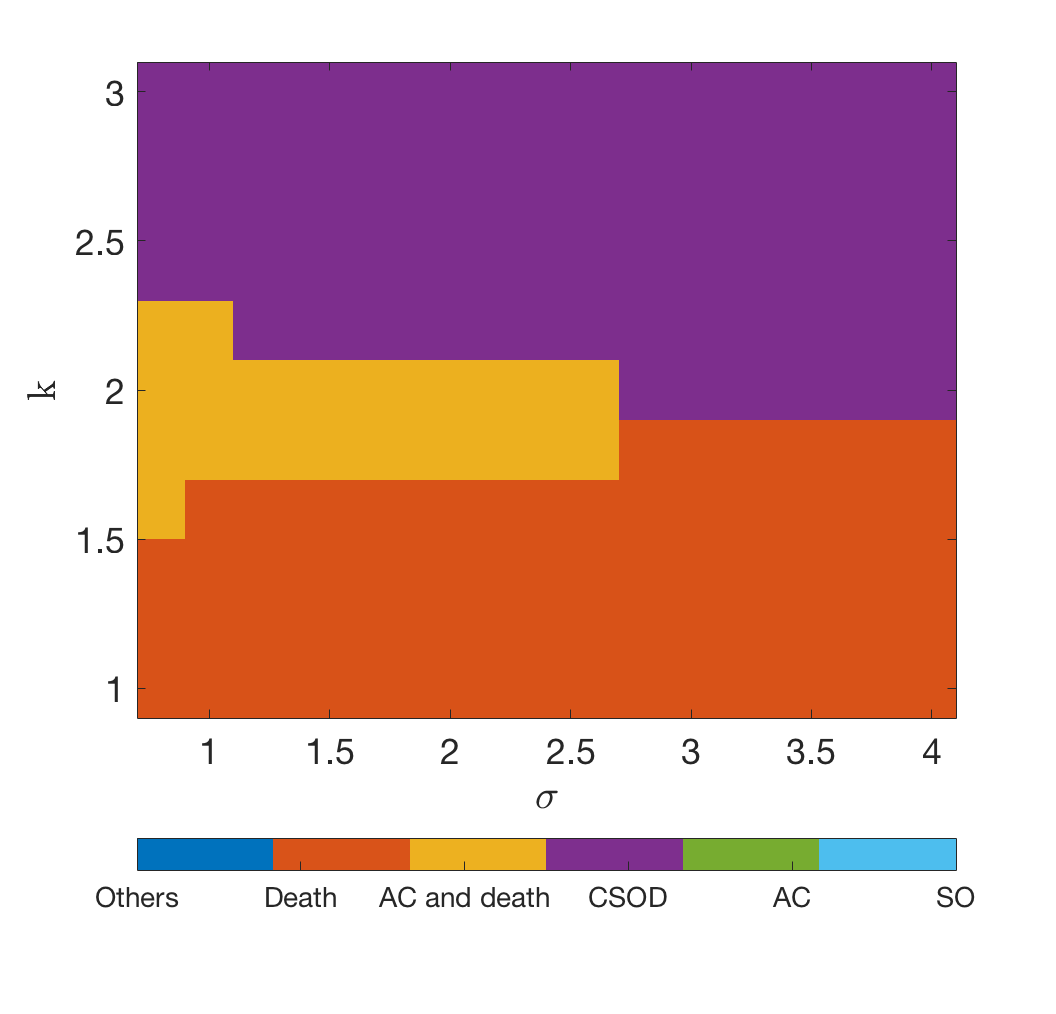
\includegraphics[width=\textwidth]{Xinzhu Section/2dlat16_sqrt(18).png}
    \caption{Link distance $l=\sqrt{18}$.}
    \end{subfigure}

    \caption{Link distance increases from $\sqrt{5}$ to $\sqrt{18}$. The region of amplitude chimera and death is gradually replaced by a region of synchronised oscillation and death.}
    \label{fig:b link distances and parameter searches}
\end{figure}

\section{Looking for Chaotic Behaviour}\label{section:chaos}
Sensitivity to initial conditions is an import consideration when modelling population dynamics. In chaotic systems small perturbations in populations may have drastic effects on medium to long term dynamics. Hence, the possibility of chaotic behaviour is an important consideration. \\ \\
Exploring the $\{ k,\sigma \} -$parameter space and different network sizes and topologies, the $0-1$ test was used to to identify whether a node was displaying chaotic behaviour or regular dynamics. As usual initial conditions were drawn randomly from a uniform distribution between $0$ and $0.4$. If the $0-1$-test statistic took a value of $0$ the behaviour was regular and if it had a value of $1$ then behaviour behaviour was chaotic \cite{gottwald20160}. \\ \\ \colorbox{yellow}{More detail on this/appendix?} Choosing values of $k$ above the Hopf bifurcation value and varying in it the range $[1.6,8]$, while varying $\sigma$ in $[10^{-6},10]$, heatmaps of the $0-1$-test results for the first node of each system were produced (example in Figure \ref{fig: no chaos heatmaps}) and no chaos was observed in any system of networks for sizes between 2 and 15 nodes.

\begin{figure}[h]
    \centering

    \begin{subfigure}[b]{0.2\linewidth}
        \centering
        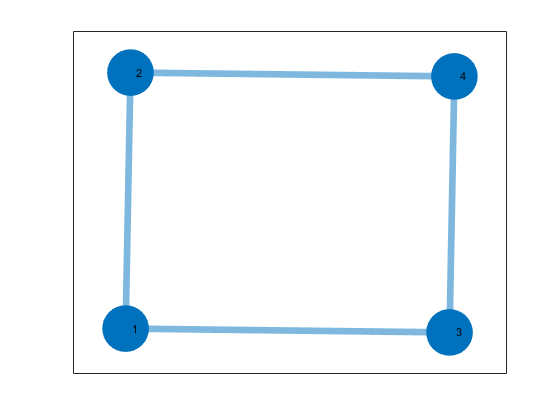
\includegraphics[width=\textwidth]{Chaos Stuff/4n_lattice.png}
        \caption{4 node lattice}
        \label{fig: 4 node lattice}
    \end{subfigure}
    \hfill
    \begin{subfigure}[b]{0.2\linewidth}
        \centering
        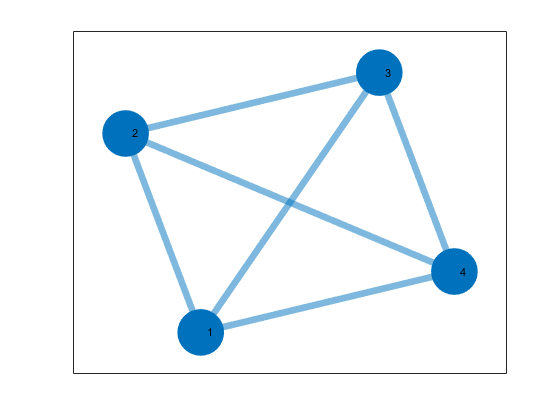
\includegraphics[width=\textwidth]{Chaos Stuff/4n_full.png}
        \caption{4 node fully connected}
        \label{fig: 4 node full}
    \end{subfigure}
    \hfill
    \begin{subfigure}[b]{0.2\linewidth}
        \centering
        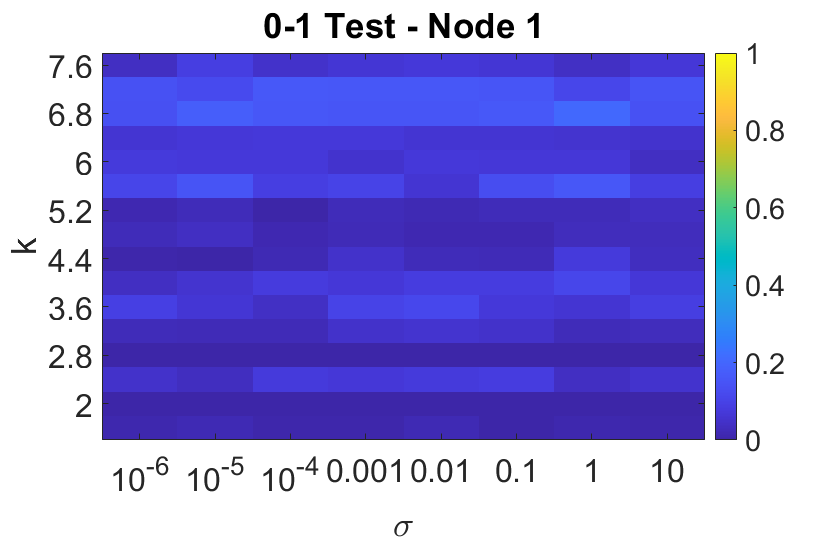
\includegraphics[width=\textwidth]{Chaos Stuff/node1_4_lattice.png}
        \caption{Heatmap 4 node lattice}
        \label{fig:4 node lattice heatmap}
    \end{subfigure}
    \hfill
    \begin{subfigure}[b]{0.2\linewidth}
            \centering
            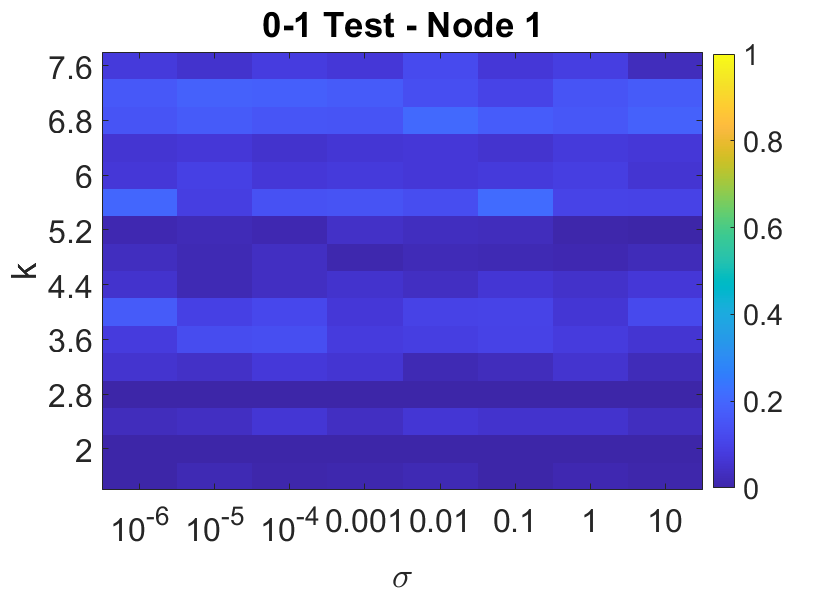
\includegraphics[width=\textwidth]{Chaos Stuff/node1_4_full.png}
            \caption{Heatmap fully-connected}
            \label{fig:4 node full heatmap}
    \end{subfigure}
    \label{fig: no chaos heatmaps}
    \caption{Simple networks tested for chaotic behaviour across parameter space using the $0-1$-test. No chaos is observed for any combination of parameters.}
\end{figure}
\noindent
Scaling-up to a 200 node network with a chain structure, similar to work done by Banerjee and Petrovskii in 2011 \cite{banerjee2011self} and altering some of the parameters, yielded some more interesting results. The initial conditions are modified to a Gaussian perturbations around the coexistence equilibirium fixed point \ref{eq: coexistence equilibrium}. With predator mortality rate $c$ changed to $0.9$, coupling strength $\sigma$ to $0.1$ and varying carrying-capacity $k$ in the range $20-40$, chaotic dynamics are observed.  \\ \\

\begin{figure}[h]
    \centering
    \begin{subfigure}[b]{0.32\linewidth}
        \centering
        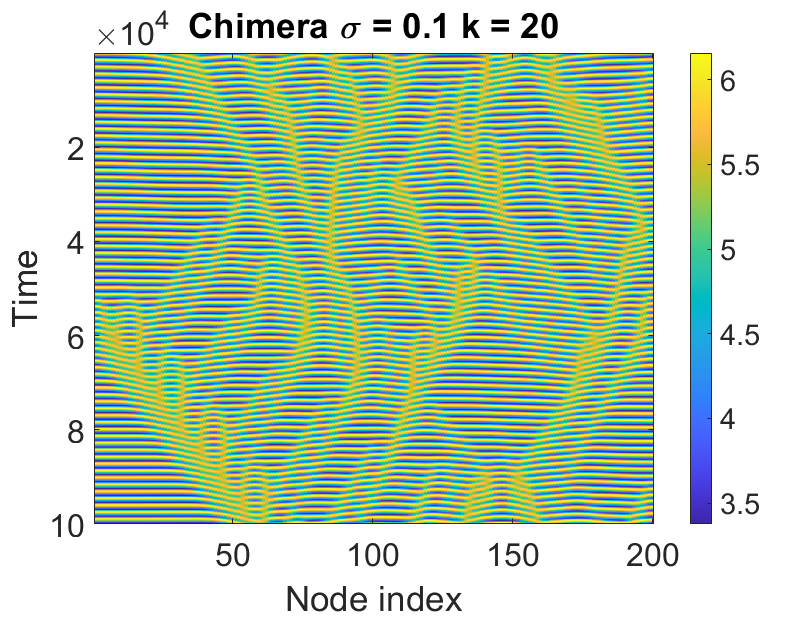
\includegraphics[width=\textwidth]{Chaos Stuff/plot1.png}
        \label{fig: k20traj}
    \end{subfigure}
    \hfill
    \begin{subfigure}[b]{0.32\linewidth}
        \centering
        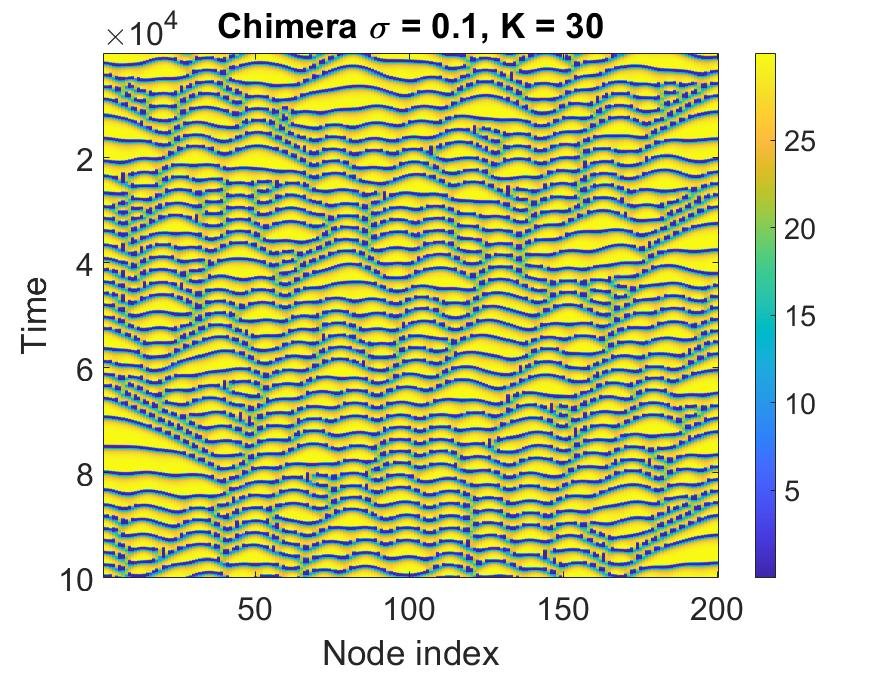
\includegraphics[width=\textwidth]{Chaos Stuff/k30chim.jpg}
        \label{fig: k30traj}
    \end{subfigure}
    \hfill
    \begin{subfigure}[b]{0.32\linewidth}
        \centering
        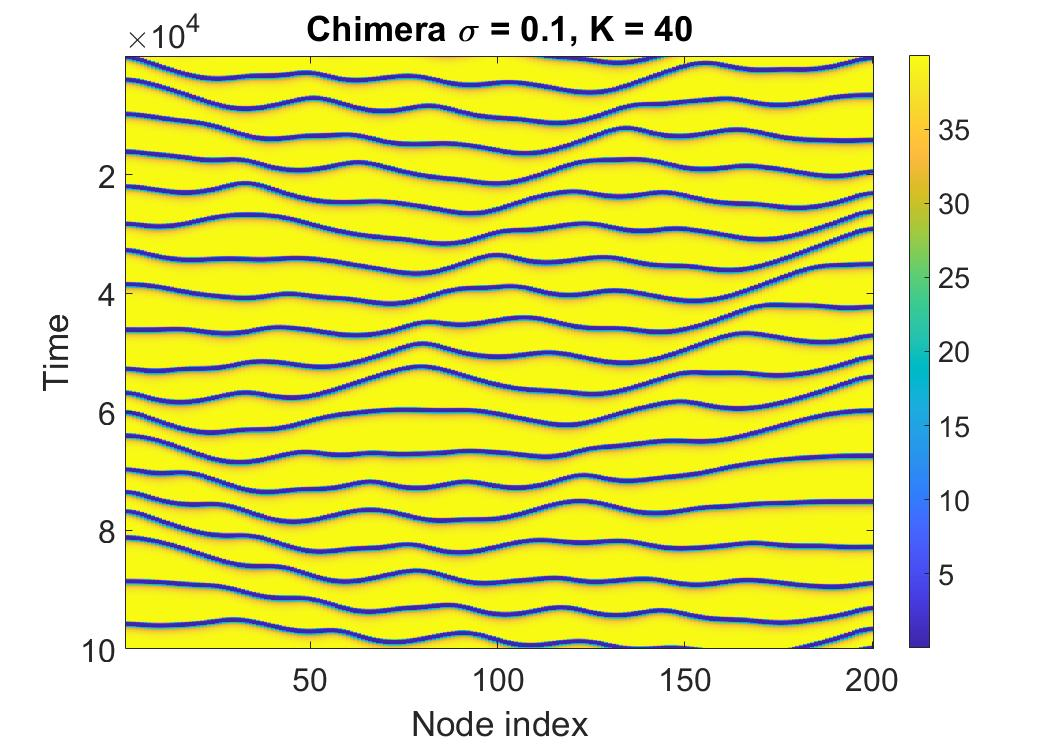
\includegraphics[width=\textwidth]{Chaos Stuff/k40chim.jpg}
        \label{fig:k40traj}
    \end{subfigure}
    \hfill
    \begin{subfigure}[b]{0.32\linewidth}
        \centering
        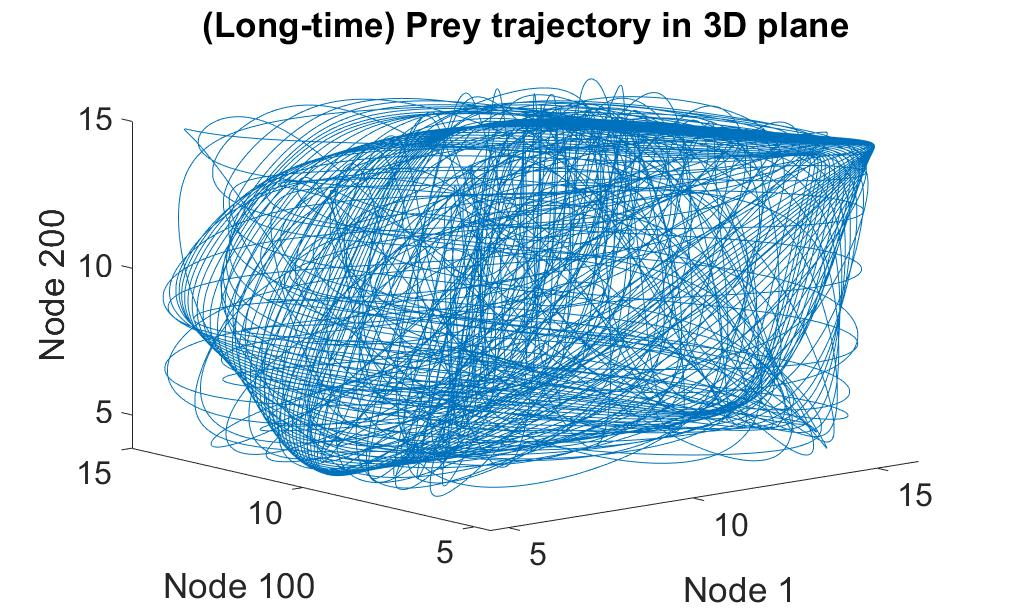
\includegraphics[width=\textwidth]{Chaos Stuff/k20traj.jpg}
        \label{fig:k20lattice}
    \end{subfigure}
    \hfill
    \begin{subfigure}[b]{0.32\linewidth}
        \centering
        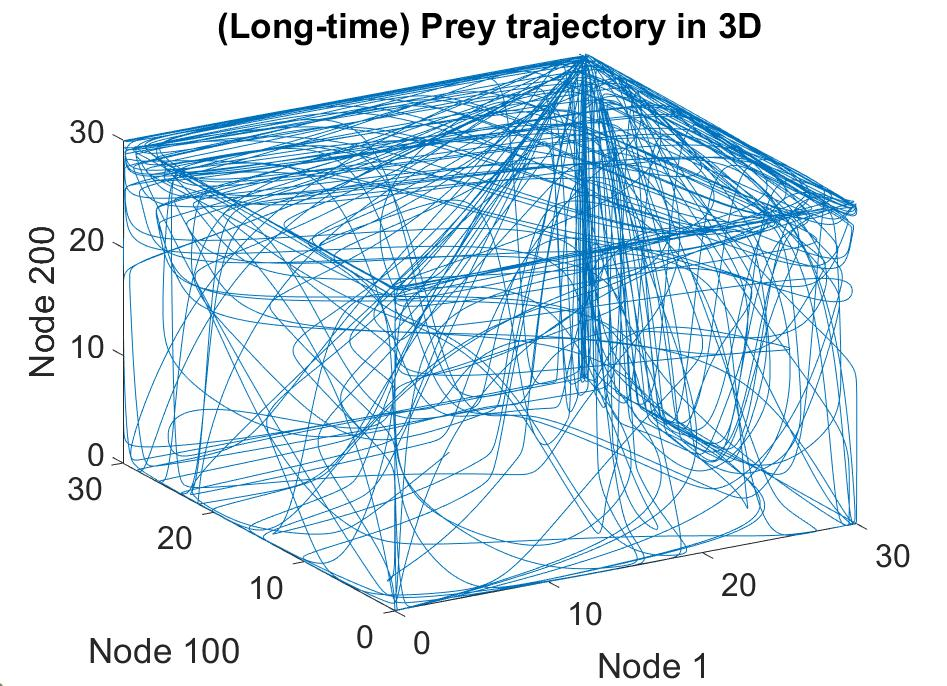
\includegraphics[width=\textwidth]{Chaos Stuff/k30traj.jpg}
        \label{fig: k30lattice}
    \end{subfigure}
    \hfill
    \begin{subfigure}[b]{0.32\linewidth}
        \centering
        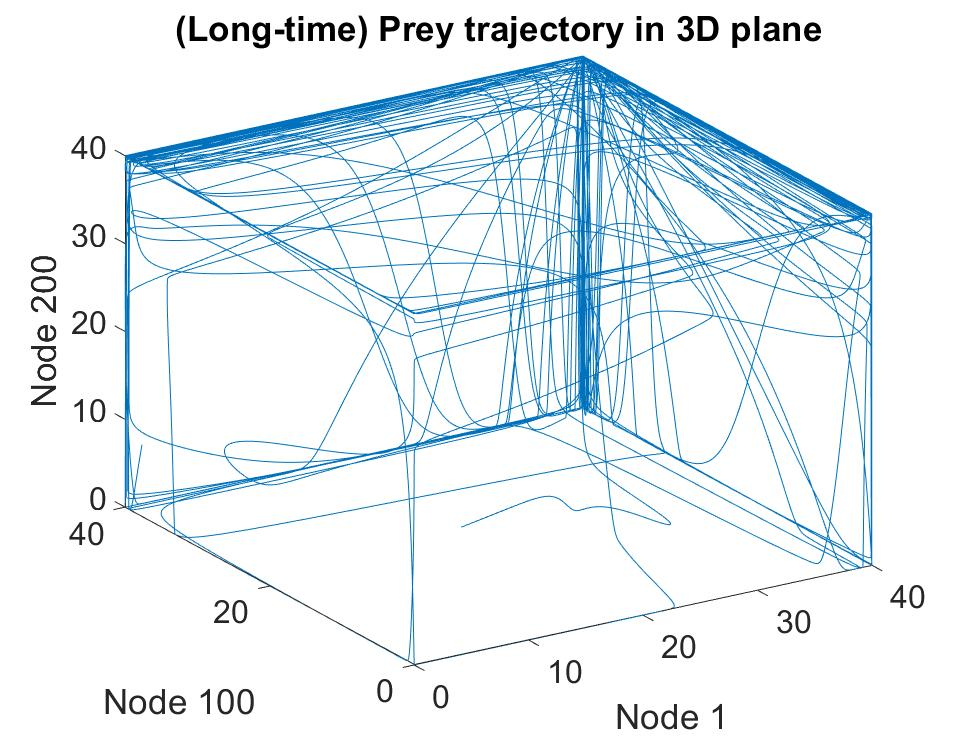
\includegraphics[width=\textwidth]{Chaos Stuff/k40traj.jpg}
        \label{fig:4 node lattice heatmap}
    \end{subfigure}
    \label{fig:k40lattice}
    \caption{The time-series of the above systems were classified as chaotic by the 0-1 test. Plots of the trajectories of the prey density of three nodes map out a cube-like 3-dimensional shape. The volume of this shape grows as the carrying capacity $k$ increases. Parallels can be drawn between this volume increase with $k$ and increasing amplitude in the single node model.}
\end{figure}
\noindent
Further increasing $k$ to $100$ the system reverts to a mixed amplitude chimera and death state as can be seen in Figure \ref{fig:k100 plot} and is no longer chaotic.

\begin{figure}[h]
    \centering
    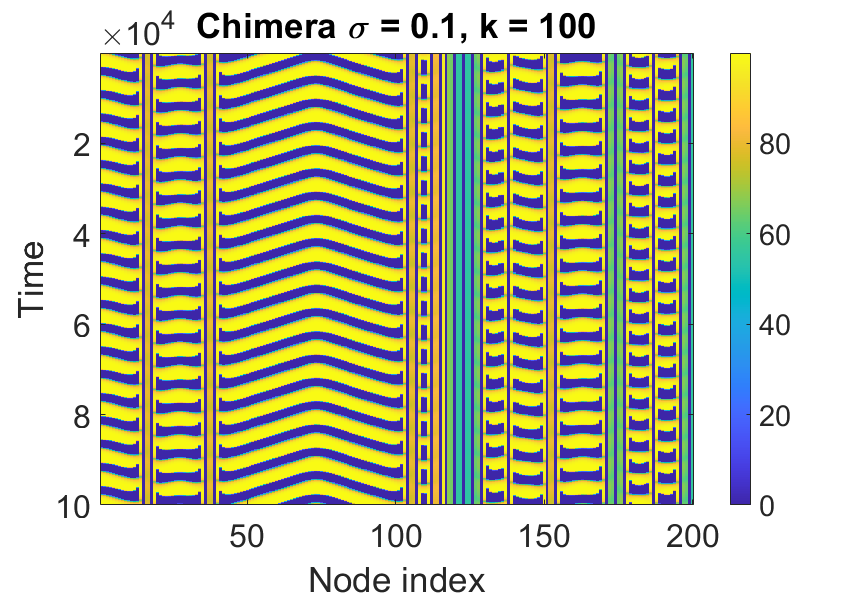
\includegraphics[width = 0.6\textwidth]{Chaos Stuff/plot4.png}
\end{figure}\label{fig:k100 plot}

\section{Case Study: Fragmentation in the Amazon rainforest}\label{section:case study}
Now we will try to understand how these results can be relevant in a real world fragmentation example.
The 2010 paper \textit{The fate of Amazonian forest fragments: A 32-year investigation}, details how the Biological Dynamics of Forest Fragments Project (BDFFP) \cite{laurance2011} has been studying the effects of fragmentation on the biota of the Amazon rainforest since 1979. This is the largest and most extensive study of its type. The area of study contains 11 square forest fragments of various sizes separated by distances of 80-650m which have been maintained throughout the study. The main focus of this project, originally titled \textit{the Minimum Critical Size of Ecosystems Project}, is to understand the effect of fragment size, which this paper finds to be vital to species richness in a fragmented landscape. This paper cites a number of findings which we seek to compare to our model results. Fragmented populations experience far higher variability than those in continuous habitats, some butterfly species have been observed to experience dramatic population explosions or \textit{hyperdynamism}, a term used to describe the increased frequency or amplitude of dynamics in fragmented habitats \cite{leidner2010does,laurance2011}. This was noted especially for small habitats with low migration rates \cite{laurance2011}. Fragmentation may give rise to unusual transitional states that would not be seen in undisturbed ecosystems \cite{terborgh2001ecological} and lastly it observes that predator populations are more vulnerable to fragmentation than prey.

% Claire's things here
\begin{figure}[H]
    \begin{subfigure}[b]{\linewidth}
    \centering
    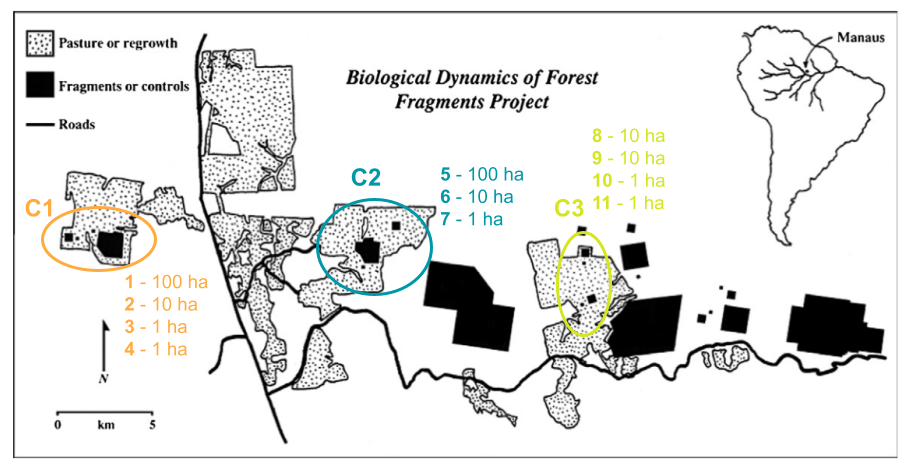
\includegraphics[width = \textwidth]{Claire Section/study_sites.png}
    \caption{Annotated study sites from \cite{laurance2011}. Unshaded areas represent intact forest and fragments represent fragments.}
    \end{subfigure}
    \hfill
    \begin{subfigure}[b]{\linewidth}
    \centering
    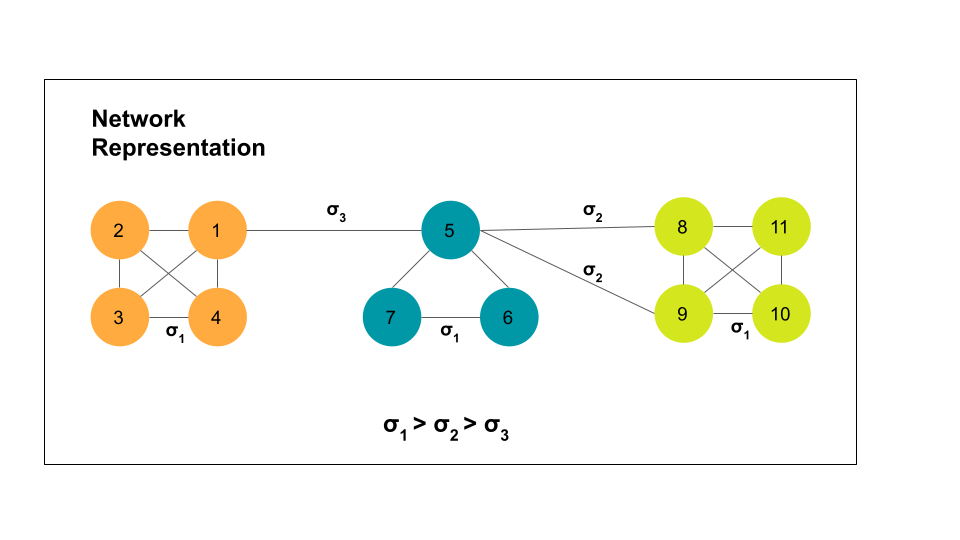
\includegraphics[width = \textwidth]{Claire Section/network_version.png}
    \caption{Network abstraction of the study}
    \end{subfigure}
    \label{fig: case study intro}
\end{figure}
\noindent To maintain some agreement with the Abram and Strogatz definition of chimera, which requires the coupled oscillators to be identical, we don't alter the carrying capacity between the study sites or the intra-cluster migration rate $\sigma_1$. Instead we only vary inter-cluster migration rates $\sigma_2$ and $\sigma_3$. This is achieved by transforming $A$ into a weighted adjacency matrix. Nodes within a cluster are connected all-to-all and, as has been observed in real ecosystems, \cite{hagen2012biodiversity} migration will mostly occur from a certain source nodes to certain sink nodes so we need only consider these connections.

\noindent The first notable result of simulating the dynamics of this model is a dependence on initial conditions become apparent. Figure \ref{fig: sensitivity to ics} shows the dynamics of four implementation s of the same system with different initial conditions. The systems exhibit quite different examples of amplitude chimera and even synchronous oscillations in one case. This is inline with \cite{laurance2011} where a sensitivity to initial conditions in population dynamics was noted and even very similar patches with similar initial conditions diverged quite significantly over time.\\  \colorbox{yellow}{Get initial conditions for the appendix and list.} \\ \colorbox{pink}{Put this in conclusion too.}

\begin{figure}[H]
    \begin{subfigure}[b]{0.5\linewidth}
     \centering
     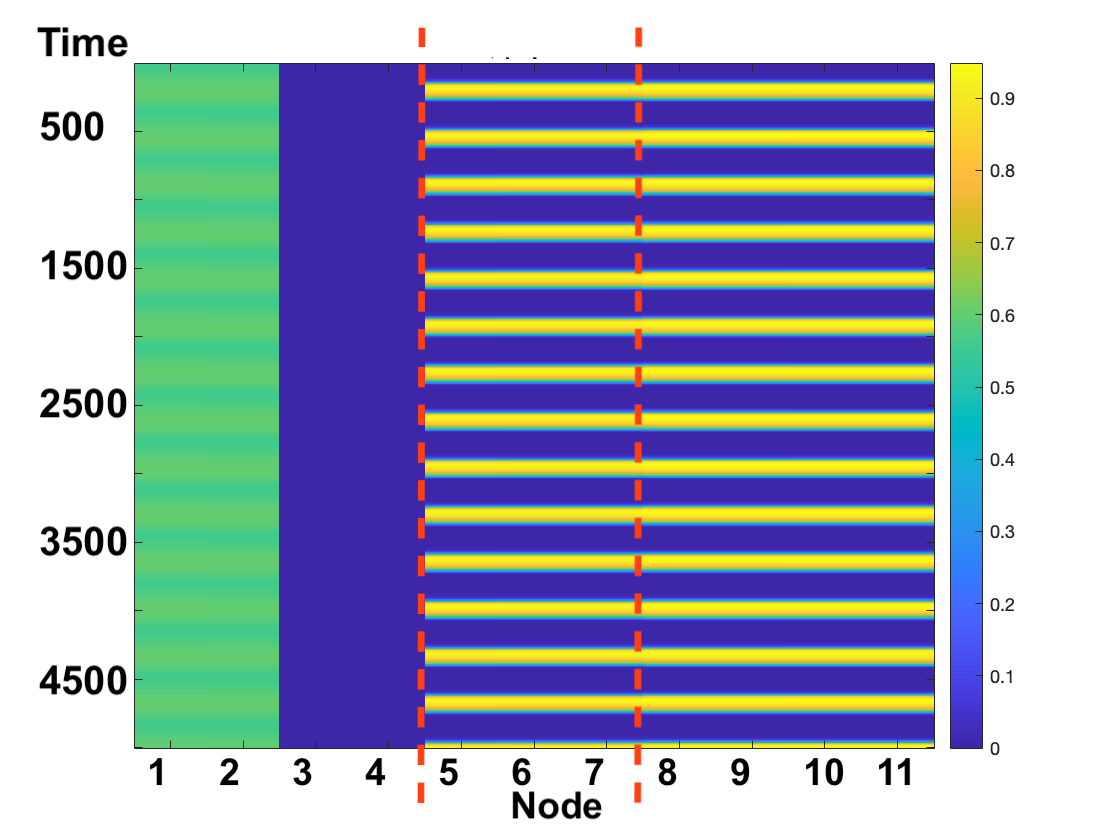
\includegraphics[width=\textwidth]{Claire Section/behavior_1.png}
     \end{subfigure}
     \begin{subfigure}[b]{0.5\linewidth}
     \centering
     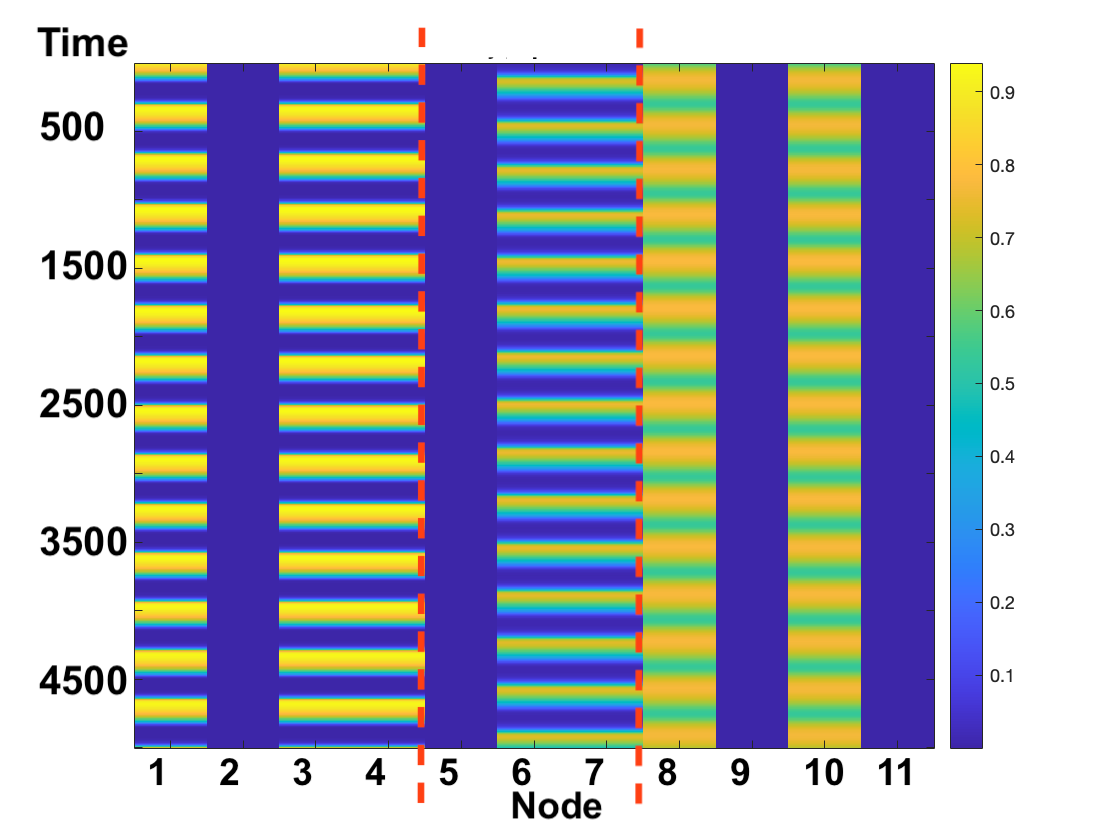
\includegraphics[width=\textwidth]{Claire Section/behavior_2-2.png}
     \end{subfigure}
     \begin{subfigure}[b]{0.5\linewidth}
     \centering
     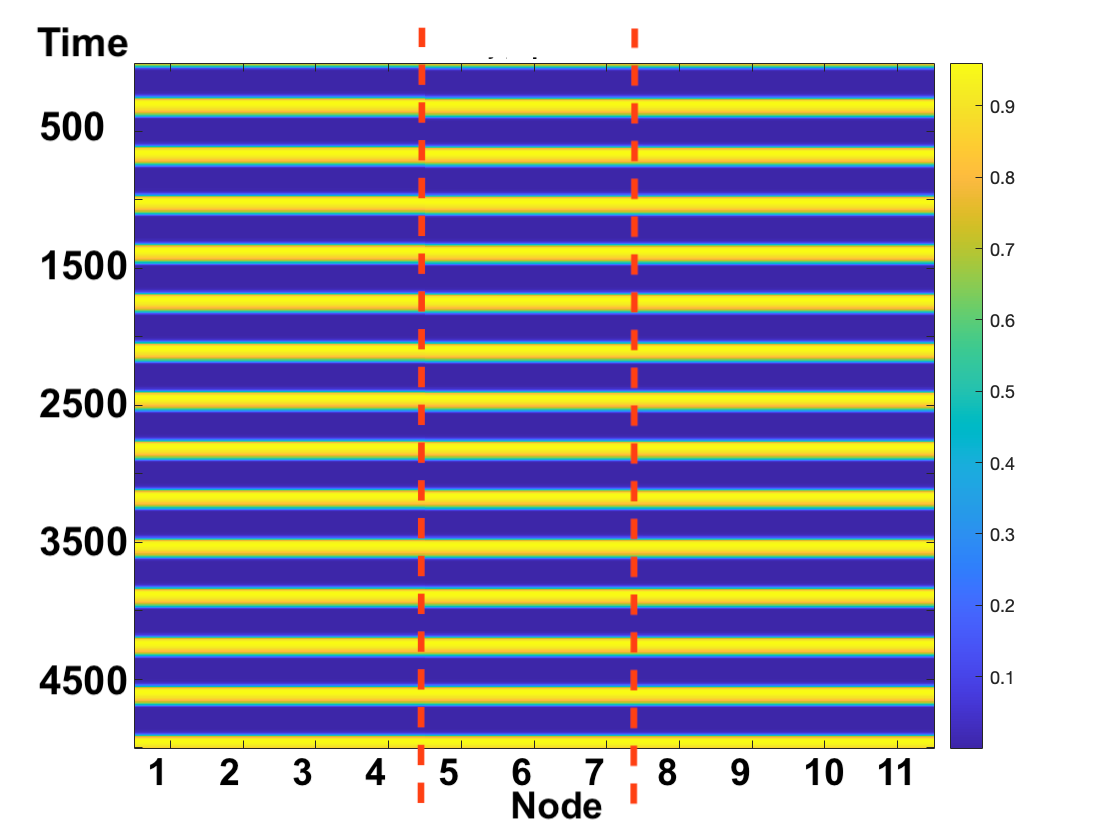
\includegraphics[width=\textwidth]{Claire Section/behavior_3.png}
     \end{subfigure}
     \begin{subfigure}[b]{0.5\linewidth}
     \centering
     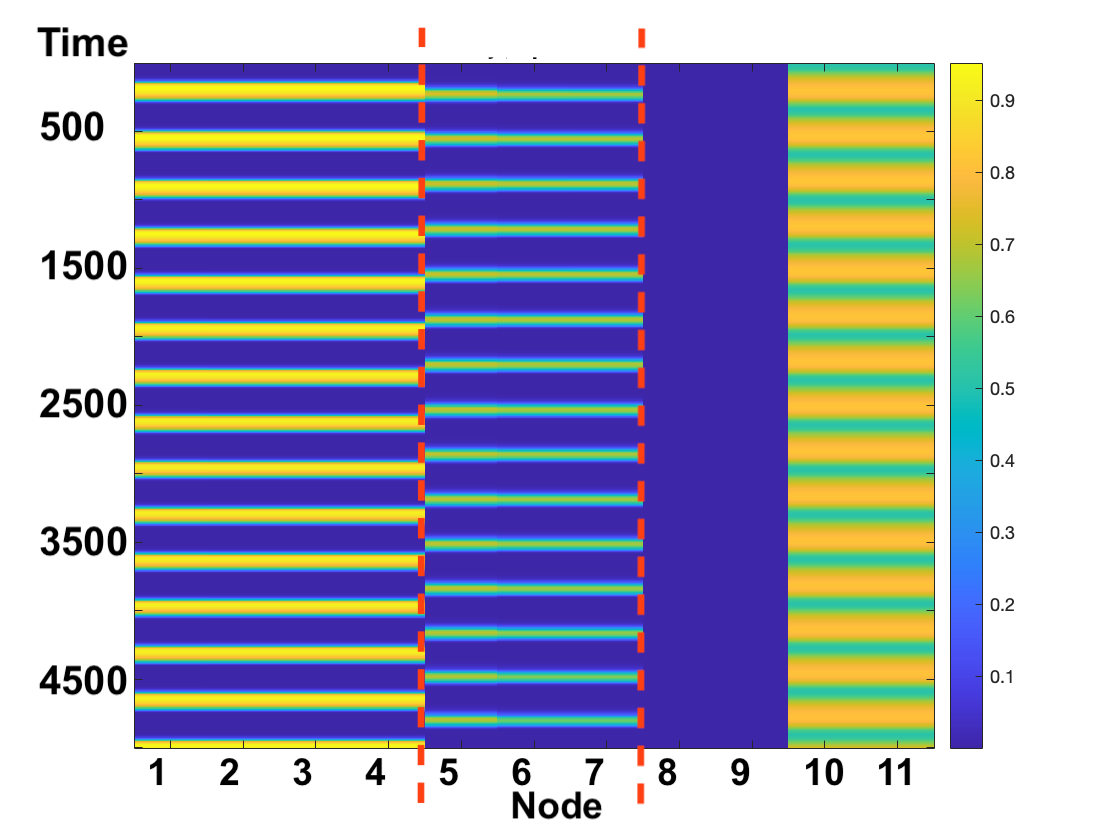
\includegraphics[width=\textwidth]{Claire Section/behavior_4.png}
     \end{subfigure}
     \label{fig: sensitivity to ics}
     \caption{Prey populations in identical habitat networks display very different instances of amplitude chimera or even synchronous oscillations depending on initial conditions.}
\end{figure}

\subsection{Progressive fragmentation}
Since fragmentation usually happens over a period of time rather than instantaneously we now study it as a process. To see how dynamics develop with progressive fragmentation of the habitat network we systematically cut off the migration between the first and second cluster by reducing $\sigma_3$ from $1$ to $0$. Observe how synchronous dynamics become incoherent for migration rates in $ \left( 0,1 \right)$ but are for $\sigma_3=1$ the system oscillates in full synchrony and for $\sigma_3=0$ the nodes in cluster one end up in death state.
\begin{figure}[H]
    \centering
    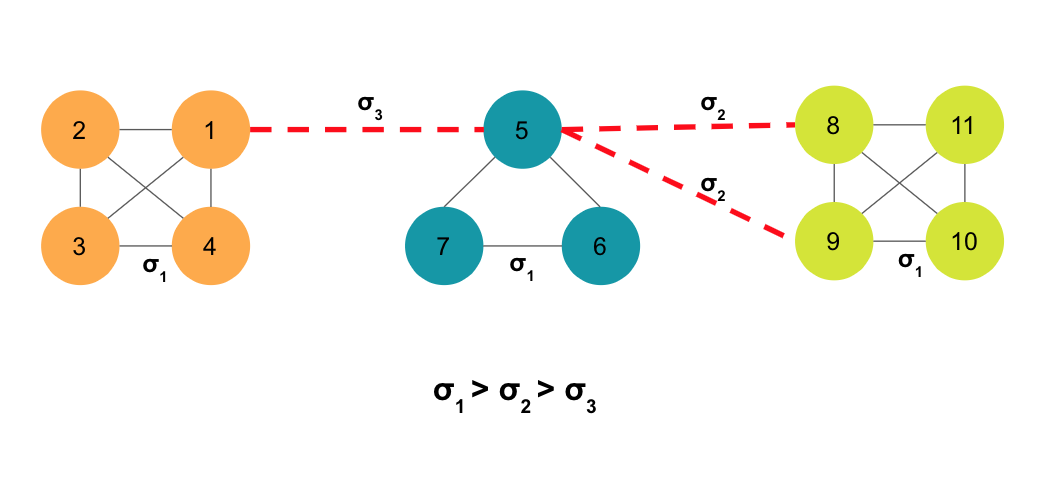
\includegraphics[width=\textwidth]{Claire Section/processive.png}
\end{figure}

\begin{figure}[H]
\centering
 \begin{subfigure}[b]{0.4\textwidth}
     \centering
     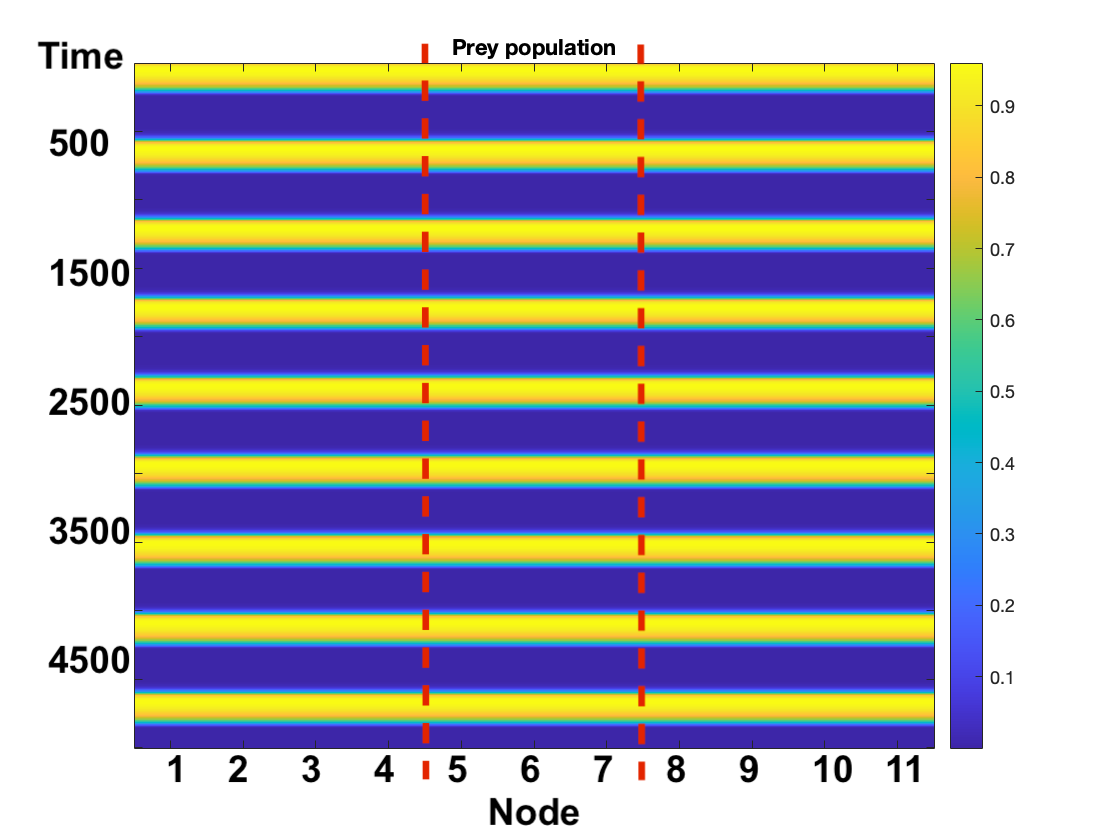
\includegraphics[width=0.9\textwidth]{Claire Section/all_mig_equal.png}
     \caption{No fragmentation}
 \end{subfigure}
 \begin{subfigure}[b]{0.4\textwidth}
     \centering
     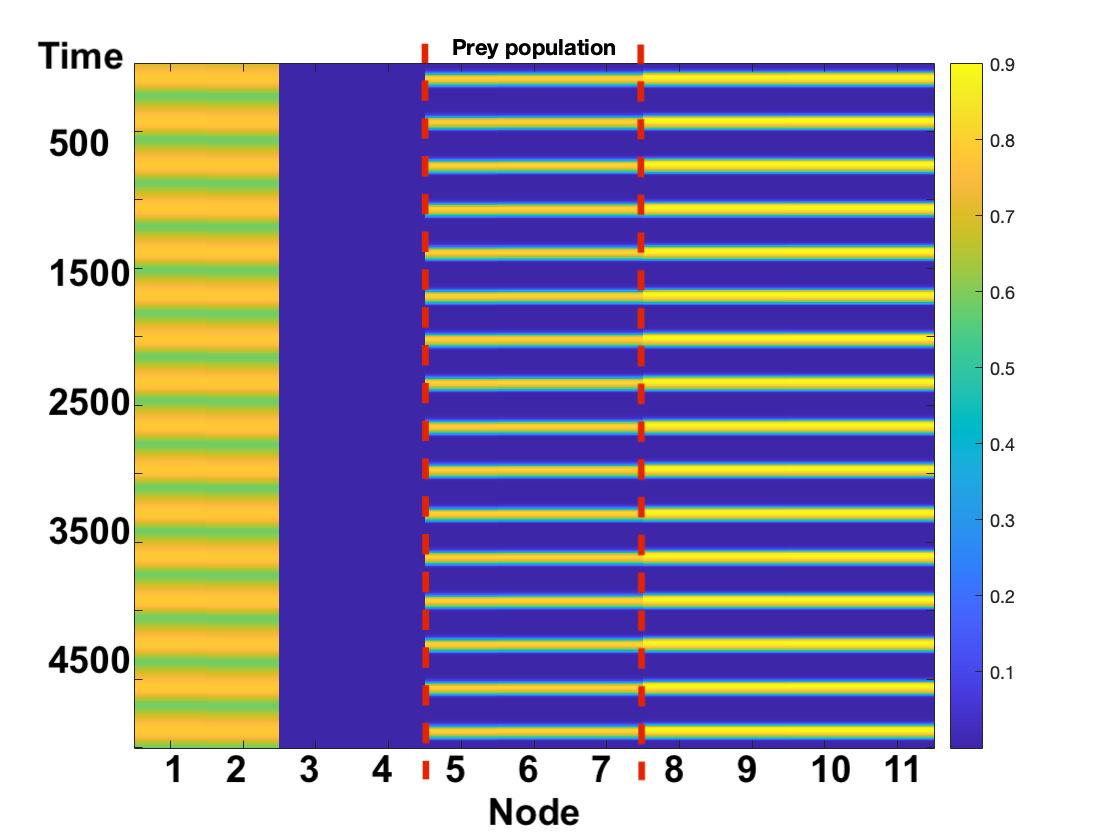
\includegraphics[width=0.9\textwidth]{Claire Section/equallow.png}
     \caption{Weights: $\sigma_3 = 0.1$, $\sigma_2 = 0.1$}
 \end{subfigure}
 \begin{subfigure}[b]{0.4\textwidth}
     \centering
     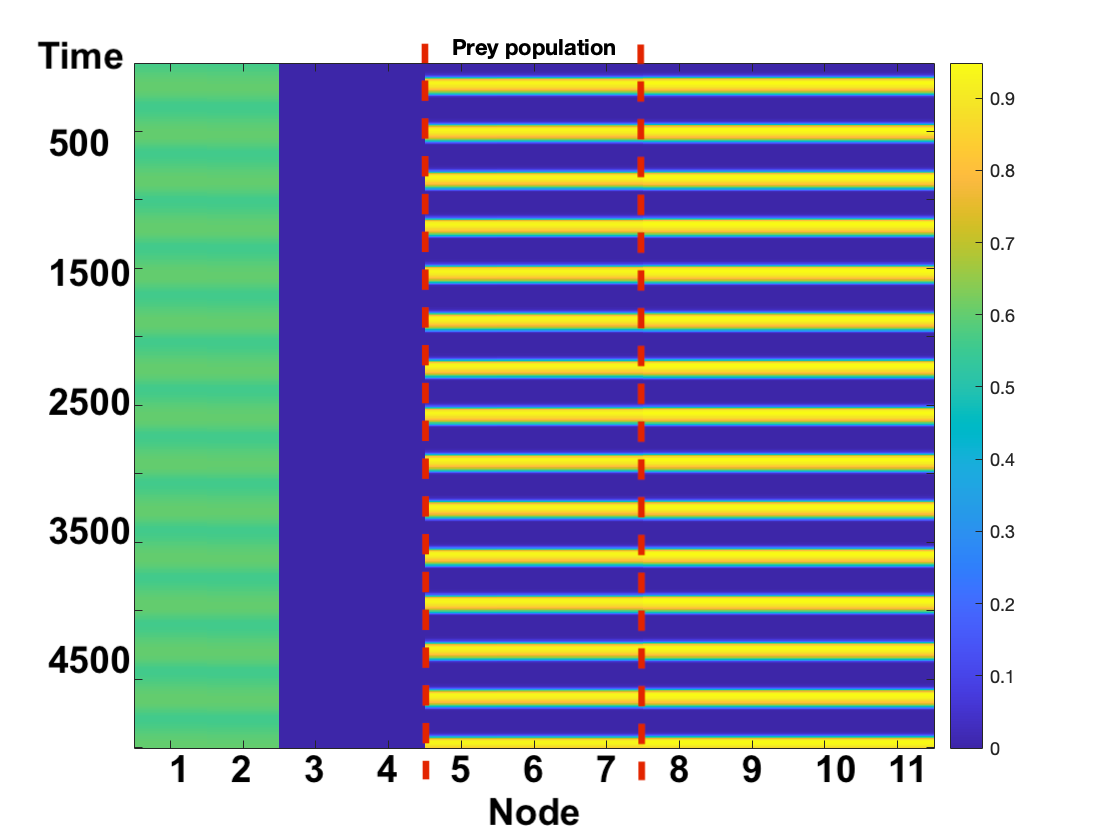
\includegraphics[width=0.9\textwidth]{Claire Section/tiered_0_01.png}
     \caption{Weights: $\sigma_3 = 0.01$, $\sigma_2 = 0.1$}
 \end{subfigure}
 \begin{subfigure}[b]{0.4\textwidth}
     \centering
     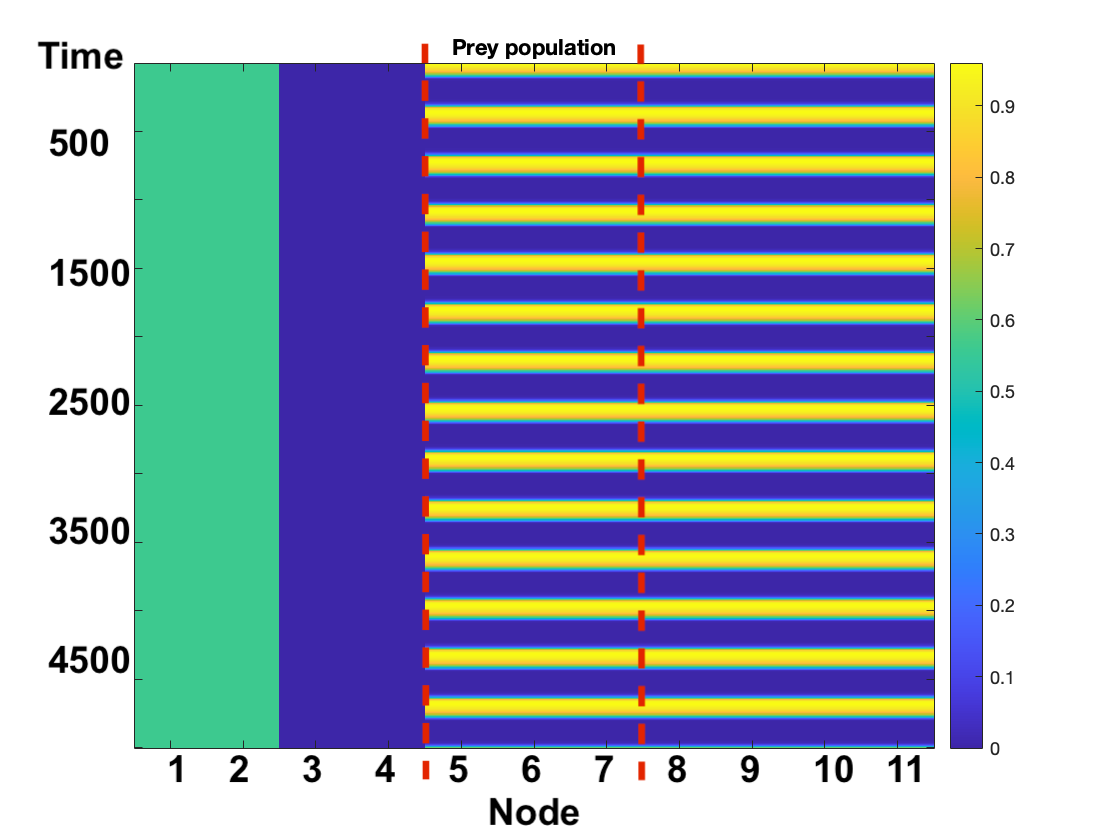
\includegraphics[width=0.9\textwidth]{Claire Section/cutoff.png}
     \caption{Cluster 1 cut off ($\sigma_3 = 0$)}
 \end{subfigure}
 \caption{Systematically cutting cluster one off from the rest of the network. Red lines indicated the three clusters.}
\end{figure}
The system in this case moves from synchronised oscillations to a mixed amplitude chimera state as the populations in the smaller cluster gradually decrease. For full cut-off we see the latter populations reduce their oscillations and approach a steady state. \colorbox{pink}{Arguably, small degree of ecosystem fragmentation could be considered healthy as it shields certain populations from shocks occurring in other parts of an ecosystem.}
\subsection{Exploring parameter space}
Laterzzz
\section{Discussion}\label{section:discussion}
In this report we have demonstrated the theoretical effects of fragmentation on a system of a habitats. We have shown that...


\printbibliography

\appendix
\section{Classifier algorithm and code}\label{appendix:classifier}
Our rough classifier works as follows: for $n$ nodes the process is run for $9000$ time steps using MATLAB's ode45() function on the system of equations \ref{fig: RMT system} and the final $1000$ entries are then extracted as a $1000 \times n$ matrix of time series and entered into a classifier function. The logic behind the algorithm is as follows: A node's temporal oscillation is analogous to the standard deviation of its time series. If this standard deviation $s$ is less than some tolerance, TOL1, then we classify the node as in a death (steady) state. If the standard deviations across the nodes very similar, having differences less than TOL2, then we conclude they have the same amplitude. We check the periodicity of the nodes using a slight modification of MATLAB's findpeaks() function. Then we proceed to classify according to Table \ref{table: chimera}

\begin{center}
 \begin{tabular}{||c | c c c c||}
 \hline
  & Synchronised Oscillations & CSOD & Amplitude Chimera & Amplitude Chimera and Death\\ [0.5ex]
 \hline\hline
 same frequency & \checkmark & \checkmark & \checkmark & \checkmark \\
 \hline
 same amplitude & \checkmark & \checkmark & \xmark & \xmark \\
 \hline
 same phase & \checkmark & \checkmark & \xmark (but spatially correlated) & \xmark (but spatially correlated) \\
 \hline
 death states present & \xmark & \checkmark & \xmark & \checkmark \\
 \hline
\end{tabular}
\end{center}


if a node is oscillating then its value is non-constant in time, hence it's standard deviation across time will be non-zero. We define a node as oscillating if and only if it's standard deviation across time is non-zero. Nodes which have the same frequency, amplitude and phase are in synchrony but if only their frequencies are the same then we have amplitude chimera. In this case, we set the tolerance for a node to be in a zero state, TOL1, to $10^{-4}$ and we set the tolerance for difference between node amplitudes and period to TOL1$=$TOL2$=10^{-1}$.

\colorbox{yellow}{add flowchart (in laptop case)}


After tuning the model on several systems with known behaviour, values of TOL1$=10^{-1}$ and TOL2$=$TOL3$=10^{-2}$ were selected.

\section{Looking for Chaos} \label{appendix:chaos}
The $0-1$ test, introduced by Gottwald and Melbourne in 20014 \cite{gottwald2004new} is an alternative test to calculating the maximal Lyapunov exponent for identifying chaotic behaviour and can be applied to any time series. The test needs no supplementary information about the underlying time series and the data needs no pre-processing. It uses recent developments in ergodic theory \cite{gottwald2004new } so was implemented as a bit of a "black box" algorithm for the purposes of this study.  The system was allowed to run for a long period of time \colorbox{yellow}{200,000} to reduce the effect of initial conditions and allow nodes to settle into more long-term behaviours. A time-series of the last last 100,0000 steps for first node in the system was then extracted and the $0-1$-test implemented on that.

\section{Linear Stability Analysis} \label{appendix:lsa}



\end{document}
